% ACM Computing Surveys (CSUR) submission template (acmsmall).
% nonacm disables the conference/copyright block during pre-submission
% review; the ACM Editorial Office sets the final block at acceptance.
%
% Review model: CSUR uses single-anonymous (single-blind) peer review.
% Verified 2026-05-15 from three ACM sources:
%   1. CSUR Author Guidelines (https://dl.acm.org/journal/csur/author-guidelines)
%      require the manuscript to carry "Author names and affiliations"
%      and "A footnote on the first page should acknowledge funding
%      sources", and grant authors "the option to identify non-preferred
%      reviewers" -- all signatures of single-anonymous review.
%   2. ACM Peer Review Policy (https://www.acm.org/publications/policies/peer-review)
%      and its FAQ confirm that ACM publications use single or double
%      anonymous review; CSUR's author-facing instructions specify the
%      single-anonymous variant.
%   3. CSUR has not been listed as a venue running an experimental
%      (zero-anonymous or open) peer-review model.
% Author identities therefore remain visible to reviewers; reviewer
% identities remain hidden from authors. No 'anonymous' documentclass
% option is required for the standard CSUR submission flow.
%
% If, after assignment, the handling editor instructs a double-anonymous
% review, switch by replacing the documentclass line with:
%   \documentclass[acmsmall, nonacm, screen, anonymous]{acmart}
% which suppresses author names, affiliations, acknowledgements, and
% self-identifying funding statements in the rendered PDF.
\documentclass[acmsmall, nonacm, screen]{acmart}

% Document-specific packages (acmart already loads amsmath, amssymb,
% graphicx, xcolor, hyperref, cite, amsthm internally).
\usepackage{booktabs}
\usepackage{multirow}
\usepackage{array}
\usepackage{tabularx}
\usepackage{rotating}
\usepackage{longtable}
\usepackage{colortbl}
\usepackage{pdflscape}
\usepackage{placeins}
\usepackage{tikz}
\usetikzlibrary{positioning, arrows.meta, shapes.geometric, calc, fit, backgrounds}

\newtheorem{definition}{Definition}

% Placeholder marker for items that depend on the second-coder /
% expanded-corpus analysis still in progress. Renders prominently so
% it cannot be missed in proof.
\newcommand{\TODO}[1]{\textbf{\textcolor{red}{[TODO: #1]}}}

% Dimension header colours matching taxonomy diagram
\definecolor{d1col}{RGB}{26,82,118}
\definecolor{d2col}{RGB}{30,132,73}
\definecolor{d3col}{RGB}{125,60,152}
\definecolor{d4col}{RGB}{183,119,13}
\definecolor{d5col}{RGB}{176,58,46}
\definecolor{d6col}{RGB}{17,122,139}
\definecolor{d7col}{RGB}{99,57,116}
\definecolor{rowgray}{gray}{0.94}

% ---------------------------------------------------------------
% ACM Journal metadata
% ---------------------------------------------------------------
\acmJournal{CSUR}
\acmVolume{XX}
\acmNumber{X}
\acmArticle{X}
\acmYear{2026}
\acmMonth{5}

% ---------------------------------------------------------------
% Title and authors
% ---------------------------------------------------------------
\title{A Systematic Survey and Taxonomy of Prompt Engineering
Evaluation Frameworks for Large Language Models}

\author{Rohith Reddy Bellibaltu}
\orcid{0009-0003-6083-0364}
\affiliation{%
  \institution{Florida International University}
  \city{Miami}
  \state{Florida}
  \country{USA}
}
\email{rohithreddybc@gmail.com}

\author{Pratyush Jena}
\orcid{0009-0002-5910-9847}
\affiliation{%
  \institution{Florida International University}
  \city{Miami}
  \state{Florida}
  \country{USA}
}
\email{pjena001@fiu.edu}

\author{Triveni Morla}
\orcid{0009-0007-2485-1909}
\affiliation{%
  \institution{Florida International University}
  \city{Miami}
  \state{Florida}
  \country{USA}
}
\email{tmorla@fiu.edu}

\author{Wenbin Zhang}
\orcid{0000-0003-3024-5415}
\affiliation{%
  \institution{Florida International University}
  \city{Miami}
  \state{Florida}
  \country{USA}
}
\email{wenbin.zhang@fiu.edu}

\renewcommand{\shortauthors}{Bellibaltu et al.}

% ---------------------------------------------------------------
\begin{document}
% ---------------------------------------------------------------

% ---------------------------------------------------------------
\begin{abstract}
Prompt engineering evaluation lacks a shared conceptual frame. Two
papers can report improvements on the same prompting technique using
methods, metrics, and scopes that are internally consistent yet
mutually incomparable, not because either study is poorly designed,
but because the surveyed literature has not converged on what should
be measured or how. We trace this to two unresolved measurement-theory
tensions: construct validity vs.\ measurement reliability, and
reference-anchored vs.\ judgment-anchored evaluation.

We propose a seven-dimensional taxonomy (D1--D7: evaluation method,
task scope, metric type, automation level, evaluation scope,
robustness, reproducibility) and apply it to a 152-paper PRISMA~2020
corpus from six databases (79-paper primary set plus four
coverage-repair expansion rounds). The taxonomy identifies three
recurring archetypes supported by convergent unsupervised criteria
($k$-means, hierarchical, GMM, spectral; BIC-minimum at $k=3$;
bootstrap-stable membership) and labelled descriptively
(Benchmark-Automation, Judge-Mediated, Expert-Anchored). Archetypes
constructed from D1 and D4 statistically predict D6 and D7
properties not used in construction ($\chi^2$ test, Cram\'{e}r's
$V = 0.21$ and $0.33$ respectively), evidence that the taxonomy
carries information beyond surface organization. We also report
three corpus-prevalent failure modes (FM1: Construct Mismatch, 7.2\%;
FM2: Unpinned Judge, 16.4\% of corpus and 83.3\% of the LLM-judge
subgroup; FM3: Single-Phrasing Generalization, 29.6\%) where an
evaluation's dimensional configuration does not support its stated
claims.

Three patterns emerge. The dominant archetype (Benchmark-Automation,
66.4\% of the corpus) occupies the high-reliability, narrow-validity
region: well-suited to tasks with ground-truth answers but
under-specifying the construct for open-ended generation. The
Judge-Mediated archetype (17.1\%) addresses this gap at the cost of
judge-model reliability concerns the surveyed corpus has not yet
managed with a shared calibration protocol. Robustness and
contamination-resistant evaluation remain minority practices.

The taxonomy is not a new evaluation method. We propose it as one
organizing scheme for prompt engineering evaluation through a
measurement-theoretic lens; whether the resulting vocabulary
(D1--D7, FM1--FM3, archetype labels) proves useful for disclosing
and comparing evaluation methodology is for the community to decide.
A companion seven-question checklist accompanies the taxonomy as a
practitioner aid.
\end{abstract}

\keywords{prompt engineering, large language models, evaluation
frameworks, taxonomy, systematic review, LLM evaluation, benchmark
evaluation, LLM-as-judge, evaluation design, evaluation checklist,
NLP benchmarks, automation level, task scope, metric selection,
evaluation reproducibility}

\begin{CCSXML}
<ccs2012>
   <concept>
       <concept_id>10010147.10010178.10010187</concept_id>
       <concept_desc>Computing methodologies~Natural language processing</concept_desc>
       <concept_significance>500</concept_significance>
       </concept>
   <concept>
       <concept_id>10010147.10010257.10010282</concept_id>
       <concept_desc>Computing methodologies~Language resources</concept_desc>
       <concept_significance>300</concept_significance>
       </concept>
   <concept>
       <concept_id>10002951.10003317.10003331</concept_id>
       <concept_desc>Information systems~Evaluation of retrieval results</concept_desc>
       <concept_significance>300</concept_significance>
       </concept>
   <concept>
       <concept_id>10002944.10002946</concept_id>
       <concept_desc>General and reference~Surveys and overviews</concept_desc>
       <concept_significance>300</concept_significance>
       </concept>
   <concept>
       <concept_id>10002951.10003227.10003233.10003235</concept_id>
       <concept_desc>Information systems~Test collections</concept_desc>
       <concept_significance>100</concept_significance>
       </concept>
 </ccs2012>
\end{CCSXML}

\ccsdesc[500]{Computing methodologies~Natural language processing}
\ccsdesc[300]{Computing methodologies~Language resources}
\ccsdesc[300]{Information systems~Evaluation of retrieval results}
\ccsdesc[300]{General and reference~Surveys and overviews}
\ccsdesc[100]{Information systems~Test collections}

\maketitle

% ---------------------------------------------------------------
\section{Introduction}
\label{sec:introduction}
Within roughly four years, large language models (LLMs) have moved
from academic novelties into foundational components of production
software systems. That period has also generated substantial research
on prompt engineering (PE), the practice of crafting natural language
inputs to elicit reliable, useful model outputs without modifying
weights~\cite{liu2021pretrain, schulhoff2024prompt}. Chain-of-thought
prompting, retrieval-augmented generation, automated prompt
optimization, and dozens of related techniques have been proposed,
evaluated, and deployed across tasks as varied as arithmetic reasoning
and clinical decision support~\cite{wei2022chain, lewis2020retrieval, sahoo2024systematic}.

A concrete scenario shows why evaluation practice matters. Consider
a chain-of-thought variant for medical differential diagnosis.
Study~A evaluates it on MedQA with exact-match accuracy
(D1=Benchmark, D3=Task-specific, D4=Automated); Study~B evaluates
the same technique with GPT-4 as a clinical scoring judge on a
different question set (D1=LLM-as-Judge, D3=LLM-judge, D4=Automated).
Both report improvements over their baselines, but a clinician
choosing between them cannot combine the results: Study~A's
exact-match accuracy does not capture the reasoning quality or
safety properties clinical deployment requires; Study~B's judge
score is uninterpretable relative to clinical ground truth without
a calibration experiment. Neither study fails internally; both
results are limited by an evaluation ecosystem without a shared
vocabulary for describing what each measured, which tradeoffs each
accepts, and under what conditions results transfer across labs.
The same pattern (internally consistent, mutually incomparable
evaluations) appears throughout the broader
literature~\cite{chang2023survey, guo2023evaluating}. Proposing a
candidate vocabulary in the form of a seven-dimensional taxonomy
grounded in measurement theory, and testing whether it organizes the
literature usefully, is the primary contribution of this paper.

\subsection*{Contribution}

This paper is a structured reorganization of existing prompt
engineering evaluation practice into a measurement-theoretic frame,
together with the empirical work needed to test whether the
reorganization is well-posed. Concretely, the contribution is four
items, each independent and individually verifiable:

\begin{enumerate}
\item \textit{A seven-dimensional codebook (D1--D7).} A reproducible
operationalization of evaluation-method, task-scope, metric-type,
automation-level, evaluation-scope, robustness, and reproducibility
choices into mutually exclusive subcategories at each dimension, with
inter-rater Cohen's $\kappa$ of 0.76--0.92 on a dual-coded subsample
of $\geq38$ papers (Section~\ref{subsec:coding_reliability}).

\item \textit{A measurement-theoretic frame.} The two-tension framing
(construct validity vs.\ measurement
reliability~\cite{cronbach1955construct, messick1995validity,
jacobs2021measurement}, and reference-anchored vs.\ judgment-anchored
evaluation) adapts existing constructs from psychometrics and ML
measurement to the PE evaluation context. The novelty is the
application and the dimensional projection, not the underlying
constructs.

\item \textit{An empirical archetype finding.} Three recurring
configurations (Benchmark-Automation, Judge-Mediated,
Expert-Anchored) account for 92.8\% of the corpus under a strict
mutual-exclusion assignment, with a silhouette coefficient of 0.398
against a random-labelling baseline of $-0.037$
(Section~\ref{subsubsec:clustervalidation}). The finding is
empirically derived from the codebook; the archetype names are
descriptive.

\item \textit{A failure-mode catalog with named exemplars.}
Three dimensional fingerprints under which a paper's configuration
does not fully support its contribution claim, each instantiated by
named corpus papers (Section~\ref{subsec:failuremodes}).
\end{enumerate}

The taxonomy is not a new evaluation method but a classification
scheme together with empirical findings on how those methods co-occur.
Three concurrent works adopt a measurement-theoretic lens for adjacent
scopes: Bean et al.~\cite{bean2025measuring} on 445 LLM benchmarks
broadly, Alaa et al.~\cite{alaa2025medical} on medical benchmarks,
and Ye et al.~\cite{ye2025psychometrics} on LLM psychometrics. Our
scope is distinct: we apply the validity/reliability tension to
prompt engineering evaluation configurations across a 152-paper PRISMA
corpus and produce a seven-dimensional codebook, archetype clustering,
and failure-mode catalog (FM1--FM3) for that scope
(Section~\ref{subsec:using}). We claim contribution on the proposed
organization and empirical analyses, not field-level priority on
measurement-theoretic LLM evaluation in general.

\subsection*{Research Questions}
\label{subsec:rqs}
This survey is organized around four research questions:
\begin{description}
\item[RQ1] \textit{(Taxonomy.)} What dimensions, if any, suffice to
classify the evaluation framework of a prompt-engineering study in a
way that exposes measurement-theoretic trade-offs? Addressed in
Sections~\ref{sec:taxonomy} and~\ref{subsec:tensions}.

\item[RQ2] \textit{(Distribution.)} What are the empirical
distributions of evaluation choices across the 152-paper corpus, and
which combinations co-occur often enough to constitute recurring
\textit{archetypes}? Addressed in
Sections~\ref{subsec:d1dist}--\ref{subsec:cooccurrence} and
\ref{subsec:archetypes}.

\item[RQ3] \textit{(Failure modes.)} Where does the taxonomy expose
specific points at which an evaluation configuration does not support
the paper's contribution claim, and how prevalent are these in the
corpus? Addressed in Section~\ref{subsec:failuremodes}.

\item[RQ4] \textit{(Tensions and gaps.)} What interpretive tensions
appear consistent with the observed configurations, and what gaps in
reporting practice does the corpus show? Addressed in
Sections~\ref{subsec:tension_scalability}--\ref{subsec:tension_reproducibility}
and the future-direction agenda of Section~\ref{subsec:agenda}.
\end{description}

We apply the taxonomy to a 152-paper PRISMA 2020 corpus (six
databases, primary set of 79 papers expanded across four
supplementary rounds; Section~\ref{sec:methodology}). Three patterns
emerge within these inclusion criteria. The modal configuration
(benchmark-based, task-specific, fully automated) occupies the
high-reliability, narrow-validity region: well-matched to tasks with
ground-truth answers, under-specified on open-ended generation. The
LLM-as-Judge cluster addresses this gap but introduces judge-model
reliability concerns the corpus does not yet manage with a shared
calibration protocol. Robustness and contamination-resistant
evaluation appear in only a small minority of papers
(Section~\ref{sec:comparison}).

\subsection*{Paper Organization}

Section~\ref{sec:related_work} reviews related work and differentiates
this paper from prior surveys. Section~\ref{sec:background} provides
background on LLMs, the prompt engineering design space, metric
families, and the five measurement-theory definitions used throughout.
Sections~\ref{sec:taxonomy}--\ref{sec:tools} introduce the two
underlying tensions, define the seven dimensions, present worked
examples and a design guide, and catalog the evaluation tool landscape.
Section~\ref{sec:methodology} describes the systematic review protocol,
dual-coding, and sensitivity analysis. Section~\ref{sec:comparison}
presents per-dimension distributions, co-occurrence patterns, recurring
archetypes, and the failure-mode catalog. Section~\ref{sec:discussion}
synthesizes findings and presents a research agenda.
Section~\ref{sec:conclusion} concludes. The Electronic Supplement
provides the evaluation-design checklist (Appendix~A), a
representative ten-paper mapping (Table~B.1), and the comprehensive
152-paper mapping (Table~C.1).


% ---------------------------------------------------------------
\section{Related Work}
\label{sec:related_work}

Three streams of prior work bear on this survey: prompt engineering
methods, LLM evaluation frameworks, and NLP taxonomies. We characterize
each stream's contribution and gaps.

\subsection{Prompt Engineering Methods and Techniques}

Interest in systematic prompt design grew once input phrasing was
shown to meaningfully shift model
outputs~\cite{brown2020gpt3}. Few-shot~\cite{brown2020gpt3} and
chain-of-thought~\cite{wei2022chain} prompting established the
foundational paradigms; zero-shot CoT~\cite{kojima2022large},
self-consistency decoding~\cite{wang2023selfconsistency},
tree-~\cite{yao2023tree} and graph-of-thought~\cite{graphofthoughts2023}
extensions with the chain/tree/graph
demystification~\cite{demystifying2024}, least-to-most
decomposition~\cite{leasttomost2022}, plan-and-solve~\cite{plansolve2023},
faithful CoT~\cite{faithfulcot2023}, many-shot
ICL~\cite{manyshot2024}, AutoPrompt's gradient
search~\cite{shin2020autoprompt}, FLAN instruction
tuning~\cite{wei2022flan}, prompt-pattern catalogs~\cite{white2023prompt},
manual-prompt studies~\cite{manualpromptnotdead2025},
RAG~\cite{lewis2020retrieval}, and automated optimization
(GEPA~\cite{gepa2025}, PromptWizard~\cite{promptwizard2024}) extend
the technique catalog. Recent automated-prompt-optimization
surveys~\cite{li2025autoprompt, ramnath2025apo} and
prompting-technique catalogs~\cite{schulhoff2024prompt,
sahoo2024systematic} organize this territory but do not address the
evaluation question: once a prompting method exists, how do you know
it worked, and by what standard?

\subsection{Evaluation Frameworks for Large Language Models}

LLM evaluation developed along its own trajectory: GLUE
\cite{wang2018glue} / SuperGLUE \cite{wang2019superglue} for NLU,
BIG-Bench \cite{srivastava2022bigbench} and BIG-Bench Hard
\cite{cot_benchmark2022} for reasoning, MMLU
\cite{hendrycks2021measuring} for multitask knowledge, and MT-Bench /
AlpacaEval \cite{zheng2023judging, dubois2024alpacaeval} for open-ended
instruction following with LLM-based judges. Reference-free and
model-based scoring \cite{multidimeval2022, instructscore2023,
beyondpointwise2025, nlgevalstatus2024}, in-context retrieval
\cite{incalm2023}, and prompt-format studies
\cite{promptformat2024} expand the design space. Ni et
al.~\cite{ni2025benchmarks} reviewed 283 benchmarks and identified
recurring problems: contamination, cultural bias, and static test
sets vulnerable to memorization. LLM-judge biases (positional,
verbosity, self-enhancement) are documented at scale by Gu et
al.~\cite{gu2025llmjudge}; Feng et al.~\cite{feng2025sage} report
that even top-performing judges fail to maintain consistent
preferences on roughly a quarter of difficult pairwise cases. The
tools are numerous; what is missing is a shared structure for
comparing across them.

\subsection{Surveys and Taxonomies in Prompt Engineering and LLM Evaluation}

Survey literature treats prompting methods and evaluation practice as
separate topics with no systematic bridge. On the PE methods side, Schulhoff et
al.~\cite{schulhoff2024prompt} catalog 58 text-only prompting
techniques with a meta-analysis but no evaluation framework; Sahoo
et al.~\cite{sahoo2024systematic} and Vatsal \&
Dubey~\cite{vatsal2024survey} organize methods by application domain
and NLP task type respectively; Liu et al.~\cite{liu2026taxonomy}
build a four-aspect taxonomy of techniques (profile/instruction,
knowledge, reasoning/planning, and output-bias reliability) that
matches our title structure closely but classifies prompts rather
than the evaluations applied to them; Wen et al.~\cite{pettax2025}
build a template-structure taxonomy; Fagbohun et
al.~\cite{fagbohun2024categorization} group techniques into
seven empirical practitioner-oriented categories; Sasaki et
al.~\cite{petaxse2025} cover
SE-specific patterns; Tian et al.~\cite{petaxdefects2025} taxonomize
prompt defects in PE-for-code; He et al.~\cite{contextengineer2025}
situate PE within ``context engineering''; Liu et al.~\cite{liu2024promptingframeworks},
published in this venue, survey \emph{prompting frameworks} in the
sense of toolkits and lifecycle structures (Data, Base, Execute, and
Service Levels) rather than evaluation frameworks; Plaat et
al.~\cite{plaat2024multistep}, also in this venue, survey
multi-step reasoning with LLMs along generation, evaluation, and
control axes; and Dong et al.~\cite{dong2022survey} provide the
foundational in-context-learning survey.

On the evaluation side, Chang et al.~\cite{chang2023survey}
organize LLM evaluation around what/where/how; Zhao et
al.~\cite{explainabilityllm2023} cover explainability evaluation;
Hou et al.~\cite{advancedllmsse2024} cover LLM-for-SE evaluation;
Gururangan et al.~\cite{inadequatebenchmarks2024} critique benchmark
adequacy; Ni et al.~\cite{ni2025benchmarks} sort 283 benchmarks into
a three-tier taxonomy; Mohammadi et al.~\cite{mohammadi2025agents}
and Yehudai et al.~\cite{yehudai2025agents} propose two- and
five-dimensional agent-evaluation taxonomies respectively; Guan et
al.~\cite{guan2025multiturn} apply a PRISMA-inspired review to
${\sim}$250 multi-turn-agent evaluation sources; Li et
al.~\cite{li2025generationjudgment} survey LLM-as-Judge along
\emph{what/how/benchmark}; Lu et al.~\cite{promptprism2025}
propose a linguistically-inspired \emph{PromptPrism} taxonomy of
prompt structure.

Three recent works adopt the same measurement-theoretic framing we use
but target different scopes:
Bean et al.~\cite{bean2025measuring} systematically review 445 LLM
benchmarks for construct validity (29 expert reviewers); Alaa et
al.~\cite{alaa2025medical} argue for construct-validity-centered
evaluation of medical LLM benchmarks specifically; and Ye et
al.~\cite{ye2025psychometrics} survey LLM evaluation through the
broader lens of psychometrics, including validation and enhancement
methodology. Kearns~\cite{kearns2026quantifying} proposes a
structured-capabilities model for quantifying construct validity
across the OpenLLM Leaderboard. Laeeq et al.~\cite{laeeq2026safepe}
propose SAFE-PE, the closest direct competitor in scope: a
multi-dimensional assessment framework for prompt engineering with
six aspects (accuracy, diversity, robustness, interpretability,
fairness, ethics); SAFE-PE targets individual prompt-level
\emph{quality scoring} (case-studied on LLaMA across summarization,
QA, and code generation), whereas the present survey targets
\emph{study-level evaluation-framework configurations} across a
152-paper PRISMA corpus. These works overlap with our
theoretical grounding but target LLM benchmarks broadly, medical
benchmarks, or psychometric methodology, not prompt-engineering
evaluation configurations specifically. None of these
centrally addresses the question we foreground: for a researcher
evaluating a specific prompting technique, which evaluation framework
should they use, and why? Answering that requires a classification
of evaluation frameworks along dimensions meaningful for PE work
specifically, which is the contribution of this survey.

\subsection{Differentiation from Prior Surveys}
\label{subsec:differentiation}

Several recent surveys overlap in topic with this paper, and a CSUR-
or similar-tier reviewer is right to ask what specifically is novel
here beyond reorganizing known evaluation practices. We answer that
question directly. Table~\ref{tab:differentiation} compares this
work to eleven closely related surveys on three axes: (1)
\textit{primary scope} (catalogs prompting methods, evaluation
methods, or both); (2) \textit{theoretical framing} (whether the
survey commits to a conceptual structure beyond a flat enumeration);
and (3) \textit{coverage of the seven dimensions} introduced in
Section~\ref{sec:taxonomy}.

\begin{table*}[!t]
\caption{Differentiation from prior surveys. ``Methods'' refers to a
catalog of prompting techniques; ``eval'' refers to a catalog of
evaluation methods, benchmarks, or metrics. ``Theoretical framing''
means commitment to a conceptual structure (e.g.\ a tension, a
paradigm, or a measurement-theoretic axis) rather than a flat
taxonomy. \checkmark{} = covered as a primary axis;
$\circ$ = mentioned but not classified along; \textendash{} = not
covered. ``This work'' uses the seven dimensions defined in
Section~\ref{sec:taxonomy}.
\textit{Takeaway:} Among the compared surveys, this paper is the only one to combine a prompting-technique catalog, an evaluation-method catalog, and an explicit measurement-theoretic frame applied specifically to prompt engineering, making its coverage structurally distinct from the eleven prior surveys included in the comparison. The closest title-overlap is with Liu et al.~\cite{liu2026taxonomy} (``A comprehensive taxonomy of prompt engineering techniques for large language models'', FCS 2026), which taxonomizes \emph{techniques}; the closest framing-overlap is with Bean et al.~\cite{bean2025measuring} and Ye et al.~\cite{ye2025psychometrics}, which apply construct-validity / psychometric framing to LLM \emph{benchmarks} (445 benchmarks, 29 reviewers) and to LLM \emph{capabilities} respectively. The present survey instead taxonomizes the seven-dimensional space of \emph{prompt engineering evaluation configurations} and provides corpus-grounded archetype clustering and failure-mode catalogs for that scope.}
\label{tab:differentiation}
\centering
\footnotesize
\begin{tabular}{p{2.6cm} p{1.4cm} p{1.9cm} p{0.55cm} p{0.55cm} p{0.55cm} p{0.55cm} p{0.55cm} p{0.55cm} p{0.55cm}}
\toprule
\textbf{Survey} & \textbf{Primary scope} & \textbf{Theoretical framing} &
\textbf{D1} & \textbf{D2} & \textbf{D3} & \textbf{D4} & \textbf{D5} &
\textbf{D6} & \textbf{D7} \\
\midrule
Schulhoff et al.~\cite{schulhoff2024prompt} & Methods & Flat catalog (58 techniques) & \textendash & \checkmark & \textendash & \textendash & \textendash & $\circ$ & \textendash \\
\midrule
Sahoo et al.~\cite{sahoo2024systematic} & Methods & Application domain & \textendash & \checkmark & \textendash & \textendash & $\circ$ & \textendash & \textendash \\
\midrule
Vatsal \& Dubey~\cite{vatsal2024survey} & Methods & NLP task type & \textendash & \checkmark & \textendash & \textendash & \textendash & \textendash & \textendash \\
\midrule
Liu et al.~\cite{liu2026taxonomy} & Methods & Profile / Knowledge / Reasoning / Reliability (output bias) & \textendash & \checkmark & \textendash & \textendash & \textendash & \textendash & \textendash \\
\midrule
Budagam et al.~\cite{budagam2024hierarchical} & Eval (prompting) & Hierarchical 5-level prompting framework, cognitive principles & \textendash & \checkmark & \textendash & \textendash & \textendash & \textendash & \textendash \\
\midrule
Chang et al.~\cite{chang2023survey} & Eval & What/where/how to evaluate & \checkmark & \checkmark & \checkmark & $\circ$ & $\circ$ & $\circ$ & \textendash \\
\midrule
Ni et al.~\cite{ni2025benchmarks} & Eval (benchmarks) & Three-tier taxonomy of 283 benchmarks & $\circ$ & \checkmark & $\circ$ & \textendash & \textendash & \textendash & \checkmark \\
\midrule
Mohammadi et al.~\cite{mohammadi2025agents} & Eval (agents) & Two-dimensional & \checkmark & \checkmark & $\circ$ & \textendash & $\circ$ & \textendash & \textendash \\
\midrule
Gu et al.~\cite{gu2025llmjudge} & Eval (LLM-judge) & Bias / reliability of LLM judges & $\circ$ & \textendash & \checkmark & \textendash & \textendash & $\circ$ & $\circ$ \\
\midrule
Bean et al.~\cite{bean2025measuring} & Eval (benchmarks) & Construct validity (445 benchmarks, 29 reviewers) & $\circ$ & \checkmark & \checkmark & \textendash & \textendash & $\circ$ & $\circ$ \\
\midrule
Ye et al.~\cite{ye2025psychometrics} & Eval (LLMs) & Psychometric validation \& enhancement & $\circ$ & \checkmark & \checkmark & \textendash & \textendash & $\circ$ & \textendash \\
\midrule
\textbf{This work} & \textbf{Eval (PE)} & \textbf{Validity / reliability tensions, archetype clustering, failure modes} & \checkmark & \checkmark & \checkmark & \checkmark & \checkmark & \checkmark & \checkmark \\
\bottomrule
\end{tabular}
\end{table*}

Three differences are central. First, among the closely related
surveys reviewed here, none centrally organizes \emph{prompt
engineering evaluation} around a measurement-theoretic frame. Bean
et al.~\cite{bean2025measuring} and Ye et al.~\cite{ye2025psychometrics}
apply construct-validity and psychometric framing respectively, but
to LLM benchmarks broadly and to LLM capabilities, not to
configurations of PE evaluation; Chang et al.'s what/where/how
decomposition is descriptive rather than tension-based. Second, none of these surveys treats robustness (D6)
and reproducibility / contamination resistance (D7) as first-class
dimensions of evaluation design; they appear, when they appear at
all, as findings inside other surveys (notably Ni et al. on
benchmark contamination and Gu et al. on judge bias). Third, prior
PE-focused surveys whose titles use similar phrasing
(Schulhoff et al., Sahoo et al., Vatsal \& Dubey, Liu et al.~2026)
catalog \emph{methods}, not \emph{evaluation frameworks}; they answer
``what prompting techniques exist'' rather than ``how those
techniques are assessed''. The title-overlap with Liu et al.~2026
is purely lexical: their four aspects (profile/instruction, knowledge,
reasoning/planning, output-bias reliability) classify prompt designs,
whereas our seven dimensions (D1--D7) classify the evaluation
configurations under which prompt designs are tested. Budagam et
al.~\cite{budagam2024hierarchical} use ``evaluation framework'' in
their title but propose a single hierarchical prompting scheme for
cognitive-complexity-aware testing, not a taxonomy of existing
evaluation practice. This survey is positioned in the gap left
by all three groups: a measurement-grounded taxonomy of PE
\emph{evaluation} that explicitly incorporates robustness and
reproducibility.

% ---------------------------------------------------------------
\section{Background}
\label{sec:background}

\subsection{Large Language Models and the Role of Prompting}

Large language models are transformer-based~\cite{vaswani2017attention}
neural networks trained on web-scale text; at sufficient scale they
handle broad task ranges without task-specific
retraining~\cite{devlin2019bert, brown2020gpt3, bommasani2021foundation}.
Practitioners interact through prompts, and surface phrasing choices
produce nontrivial output differences~\cite{sclar2023formatting,
zhou2022ape}. Prompt engineering (designing inputs to obtain
reliable, useful outputs without modifying model weights) has
developed its own benchmarks, optimization algorithms, and
taxonomies~\cite{sahoo2024systematic, schulhoff2024prompt}.

\subsection{The Prompt Engineering Design Space}

The prompting design space spans manual to fully automated:
zero-shot/few-shot~\cite{brown2020gpt3},
chain-of-thought~\cite{wei2022chain}, retrieval-augmented
generation~\cite{lewis2020retrieval}, and automated prompt optimization
via textual gradient descent~\cite{pryzant2023apo} or LLM-based
search~\cite{zhou2022ape}. The question that cuts across them (how do
you know it worked?) depends on which evaluation framework you apply;
the field has no shared vocabulary for classifying those frameworks,
and this survey provides one.

\subsection{Evaluation Metric Families}

Four metric families recur across PE evaluation. \textbf{Reference-based
metrics} score model output by surface overlap against a gold
reference (BLEU~\cite{papineni2002bleu}, ROUGE~\cite{lin2004rouge});
fast and reproducible, but weakly aligned with human judgment on
open-ended tasks~\cite{liu2023geval, repairing2022}.
\textbf{Model-based metrics} use learned semantic representations
(BERTScore~\cite{zhang2020bertscore} and related), handling paraphrase
more gracefully but still requiring a reference~\cite{chang2023survey}. \textbf{LLM-as-Judge
metrics} delegate scoring to a second language model
(G-Eval~\cite{liu2023geval}), eliminating the gold-reference
requirement at the cost of importing judge biases: positional
preference, length bias, and self-enhancement
bias~\cite{zheng2023judging, gu2025llmjudge}. \textbf{Task-specific
metrics} are purpose-built and generally do not transfer (pass@$k$
for code, exact match for factual retrieval,
RAGAS~\cite{rageval2024} for retrieval-augmented pipelines); they
are often the most meaningful for their intended task but share no
common ground across tasks. Section~\ref{sec:taxonomy} organizes
these four families along D3 (Metric Type) and threads them through
the rest of the taxonomy.

\subsection{Validity and Reliability in Evaluation}
\label{subsec:validityreliability}

We use \emph{reliability} (the consistency of a measurement under
repetition) and \emph{construct validity} (the degree to which a
score is evidence about the property it is intended to
capture)~\cite{cronbach1955construct, messick1995validity} in their
measurement-theory sense throughout. The two are not equivalent and
typically pull against each other: an exact-match comparison against
a fixed answer key is highly reliable but has narrow construct
validity for ``answer quality''; an expert panel scoring open-ended
outputs can pursue higher construct validity but is expensive,
slow to replicate, and rarely accompanied by strong inter-rater
agreement~\cite{chang2023survey}. The translation of this distinction
to ML/NLP evaluation~\cite{jacobs2021measurement,
subramonian2023takeoneforteam, liao2023designing} is the spine of the
dimensional decomposition in Section~\ref{sec:taxonomy}: a high score
on a benchmark whose construct does not match the deployment task is
evidence about the benchmark, not about the deployment property.

\subsection{Formal Definitions}
\label{subsec:definitions}

The five definitions below formalize the vocabulary used throughout;
operationalizations and empirical projections appear in
Sections~\ref{sec:taxonomy} and~\ref{sec:comparison}.

\begin{definition}[Prompt Engineering Evaluation Framework]
A prompt engineering evaluation framework $\mathcal{F}$ is a tuple
$(m,\, t,\, q,\, a,\, s,\, r,\, p)$ where each component
corresponds to a choice along one of the seven dimensions defined
in Section~\ref{sec:taxonomy}: $m$ (evaluation method, D1), $t$
(task scope, D2), $q$ (metric type, D3), $a$ (automation level,
D4), $s$ (evaluation scope, D5), $r$ (robustness reporting, D6),
and $p$ (reproducibility properties, D7). Any complete instantiation
of the tuple defines a valid evaluation configuration; the corpus
in Section~\ref{sec:comparison} is analyzed as a distribution over
such configurations.
\end{definition}

\begin{definition}[Construct Validity]
An evaluation configuration $\mathcal{F}$ has construct validity for
a target property $\pi$ to the degree that high scores under
$\mathcal{F}$ constitute genuine evidence that a model or prompting
technique achieves $\pi$ in the intended deployment context.
Construct validity is partial and degree-valued, not binary: a
benchmark measuring arithmetic accuracy has high construct validity
for arithmetic tasks and substantially lower construct validity for
claims about open-ended clinical reasoning~\cite{cronbach1955construct,
messick1995validity, jacobs2021measurement}.
\end{definition}

\begin{definition}[Measurement Reliability]
An evaluation configuration $\mathcal{F}$ is reliable if repeated
applications of $\mathcal{F}$ to the same model--prompt pair produce
scores with small variance under nominally identical conditions.
\textit{Within-run reliability} (fixed software, fixed model
snapshot) and \textit{across-time reliability} (across API revisions,
judge-model updates, or benchmark re-releases) are distinct
sub-properties; high within-run reliability does not imply
across-time reliability~\cite{subramonian2023takeoneforteam}.
\end{definition}

\begin{definition}[Reference-Anchored Evaluation]
An evaluation configuration is \textit{reference-anchored} if scoring
is determined by comparison to a stored gold answer -- an exact-match
key, a reference translation, or a passing test suite -- without
invoking a separate judge. Reference-anchored configurations have
high within-run reliability but fail when no single correct answer
exists, when the reference set is contaminated by training data, or
when the reference under-determines acceptable outputs.
\end{definition}

\begin{definition}[Judgment-Anchored Evaluation]
An evaluation configuration is \textit{judgment-anchored} if scoring
is delegated to an evaluator -- a human annotator, an expert panel,
or an LLM judge -- whose output is not pre-determined by a stored
reference. Judgment-anchored configurations can pursue construct
validity beyond what any fixed reference set supports, but they
introduce evaluator-specific biases and require explicit calibration
before scores carry cross-study interpretability~\cite{gu2025llmjudge,
feng2025sage}.
\end{definition}

% ---------------------------------------------------------------
\section{A Taxonomy of Prompt Engineering Evaluation Frameworks}
\label{sec:taxonomy}

\subsection{Two Interpretive Tensions Suggested by the Analysis}
\label{subsec:tensions}

A taxonomy of evaluation frameworks can do more than catalog choices
if a small number of organizing tensions also explain why those
choices cluster as they do. We propose two such tensions as an
\emph{interpretive frame} (formalized in
Section~\ref{subsec:validityreliability}; consistent with the corpus
patterns in Section~\ref{sec:comparison}):
(1)~\textit{construct validity} vs.\ \textit{measurement reliability}
(Definitions~2--3), and
(2)~\textit{reference-anchored} vs.\ \textit{judgment-anchored}
evaluation (Definitions~4--5). Other organizing tensions are
plausible; we choose these because they are well-established in the
measurement-theory literature
they project onto~\cite{cronbach1955construct, messick1995validity,
jacobs2021measurement} and because the seven dimensions project onto
them in identifiable ways. Whether this frame has explanatory force
beyond surface organization is an empirical question we examine in
Section~\ref{subsec:archetypes}. Figure~\ref{fig:taxonomy} positions
the dimensions; Section~\ref{sec:comparison} locates the 152 papers.

\textit{What the frame organizes.} The two tensions make three
patterns we later observe in the corpus interpretable rather than
arbitrary: D1 and D3 are entangled (Section~\ref{subsec:cooccurrence}:
Cram\'er's $V = 0.702$) because choosing a judgment locus largely
determines the metric family; benchmark-automation is the modal
configuration on closed-form tasks because automation pays near-zero
construct cost when the reference well-approximates the construct
(Section~\ref{subsec:tension_scalability}); and LLM-judge adoption
fragments because moving the judgment locus to a proprietary judge
without calibration evidence breaks across-paper comparability
(Section~\ref{subsec:tension_reference}). The frame is intended as a
low-parameter organizing account of these patterns; whether it has
explanatory force beyond organization is an empirical question we
return to in Section~\ref{subsec:archetypes}.

\subsection{From Five Dimensions to Seven}
\label{subsec:fivetoseven}

An earlier formulation used five dimensions (evaluation method, task
scope, metric type, automation level, evaluation scope). Application
to the corpus revealed two limitations: the five dimensions captured
\emph{procedural} choices but did not name two literature-recognized
first-class concerns: robustness to prompt
rephrasing~\cite{sclar2023formatting, promptsensitivity2025,
butterfly2024} and reproducibility under judge drift, API change, and
contamination~\cite{ni2025benchmarks, feng2025sage}; second, automation
level was treated as a peer dimension rather than as an operationalization
of the reliability axis. The current taxonomy adds
\textit{D6 (Robustness)} and \textit{D7 (Reproducibility and
Contamination Resistance)} and reframes \textit{D4 (Automation Level)}
as a sub-axis of reliability, making both underlying tensions
traceable through every coding decision.

Per Definition~1, an evaluation framework is fully specified by a
choice along each of D1--D7. The dimensions are conceptually distinct
(each can vary independently) but not statistically independent in
practice; the co-occurrence patterns
(Section~\ref{subsec:cooccurrence}) are a finding, not a decomposition
flaw. Table~\ref{tab:taxonomy} summarizes all seven dimensions with
subcategories, axis projection, and a representative example.

\subsection{Dimension 1: Evaluation Method}
\label{subsec:d1}

How is a prompting technique assessed? D1 projects primarily onto the
judgment-locus axis: reference-anchored at the Benchmark and Ablation
end, judgment-anchored at the Human, LLM-judge, and User-study end.
Five subcategories appear in the corpus, each indexed to a primary
strength and a primary weakness: \emph{Benchmark} (reproducible,
saturation-prone~\cite{hendrycks2021measuring, ni2025benchmarks});
\emph{Human eval} (credible for open-ended tasks, expensive and slow
to replicate~\cite{chang2023survey}); \emph{LLM-as-Judge} (scales to
open-ended outputs, imports judge bias~\cite{zheng2023judging,
dubois2024alpacaeval, gu2025llmjudge}); \emph{Ablation} (isolates
component contribution, not for cross-technique comparison);
\emph{User study} (deployment-context evidence, rare in the NLP
literature). LLM self-evaluation/self-refinement methods
(Constitutional AI~\cite{bai2022constitutional}, self-refine~\cite{madaan2023selfrefine})
do not map cleanly onto any single subcategory because evaluator and
evaluated system are the same model; we code such papers by their
dominant external evidence (typically Benchmark or LLM-judge) and
note self-evaluation as the studied mechanism.

\subsection{Dimension 2: Task Scope}
\label{subsec:d2}

What type of task is the evaluation targeting? D2 acts as a
\emph{moderator} on the validity-reliability tradeoff: the same
metric yields different validity properties depending on whether the
task admits a single gold answer or a distribution of acceptable
answers. The eight primary categories are: \emph{Reasoning}
(arithmetic, symbolic, commonsense; anchor domain for
chain-of-thought~\cite{wei2022chain}); \emph{NL generation}
(summarization, dialogue, open-ended writing); \emph{Code}
(pass@$k$ against test suites~\cite{scoT2023}); \emph{QA}
(exact match or F1); \emph{Clinical/domain}
(medical QA, legal reasoning~\cite{clinicalnlp2024});
\emph{Multilingual}~\cite{vatsal2024survey}; \emph{Agentic/tool-use}
(trajectory success~\cite{yao2024taubench}); \emph{Multimodal}
(vision-, audio-grounded~\cite{fu2023mme}).
Papers spanning multiple categories are coded \emph{Multi-task}
as a cross-category label; Agentic is a smaller active population
(4 papers) added in expansion rounds 2--3; Multimodal is defined
for framework completeness but carries no active corpus instances.

\subsection{Dimension 3: Metric Type}
\label{subsec:d3}

What is being measured, and by what means? D3 is the most direct
projection of the reference-anchored / judgment-anchored axis: the
four families introduced in §\ref{sec:background},
comprising reference-based (BLEU~\cite{papineni2002bleu},
ROUGE~\cite{lin2004rouge}), model-based (BERTScore), LLM-as-Judge
(G-Eval~\cite{liu2023geval}), and task-specific (pass@$k$, exact
match, RAGAS~\cite{rageval2024}), partition along that axis.
Calibration evidence (validation of the metric against a target
judgment on the specific task) is a D3 sub-property that becomes
methodologically central for judgment-anchored metrics
\cite{liu2023geval, gu2025llmjudge}.

\subsection{Dimension 4: Automation Level}
\label{subsec:d4}

How much human involvement does the evaluation require? D4 is a
\emph{sub-axis of reliability}: fully automated pipelines maximize
across-run consistency at the cost of any construct validity human
judgment would have added, while fully manual pipelines invert that
tradeoff. We retain D4 separately because the corpus codes it
independently of D1. The four subcategories are \emph{Fully manual},
\emph{Human-in-loop} (selective routing of borderline cases to
reviewers~\cite{ouyang2022training}), \emph{Hybrid} (automated bulk
scoring with uniform human validation on a held-out sample), and
\emph{Fully automated}; human-in-loop and hybrid are not
interchangeable, since the former applies judgment selectively on
hard cases while the latter applies it uniformly.

\begin{table*}[!t]
\caption{Seven-Dimensional Taxonomy of Prompt Engineering Evaluation
Frameworks. Each dimension projects primarily onto one of the two
underlying tensions introduced in Section~\ref{subsec:tensions}:
construct validity vs.\ measurement reliability (V/R), and
reference-anchored vs.\ judgment-anchored evaluation (R/J). D5
projects onto a third, largely orthogonal generalizability axis (G).
Any combination of subcategories across dimensions is a valid
evaluation framework configuration; co-occurrence patterns observed
in practice are reported in
Section~\ref{subsec:cooccurrence}.
\textit{Takeaway:} The seven dimensions index distinct design choices that prior surveys collapse into a single axis or omit; whether this finer resolution improves discrimination over a smaller axis set is examined empirically in Section~\ref{subsec:archetypes}.}
\label{tab:taxonomy}
\centering
\footnotesize
\begin{tabular}{p{1.8cm} p{2.7cm} p{0.6cm} p{3.8cm} p{3.4cm}}
\toprule
\textbf{Dimension} & \textbf{Subcategories} & \textbf{Axis} &
\textbf{What it captures} & \textbf{Representative example} \\
\midrule
D1 Evaluation method &
Benchmark, Human eval, LLM-as-Judge, Ablation, User study &
R/J &
The procedure used to assess prompting technique performance &
MT-Bench: LLM-as-Judge on open-ended tasks~\cite{zheng2023judging} \\
\midrule
D2 Task scope &
Reasoning, NLG, Code, QA, Clinical, Multilingual, Agentic, Multimodal, Multi-task &
mod &
The task domain that moderates the validity/reliability tradeoff &
GSM8K: arithmetic reasoning~\cite{wei2022chain} \\
\midrule
D3 Metric type &
Reference-based, Model-based, LLM-judge, Task-specific &
R/J &
The measurement approach used to score outputs (and its calibration) &
G-Eval: GPT-4 rubric scoring~\cite{liu2023geval} \\
\midrule
D4 Automation level &
Manual, Human-in-loop, Hybrid, Fully automated &
V/R &
Sub-axis of reliability: degree of human involvement &
APO: fully automated scoring~\cite{pryzant2023apo} \\
\midrule
D5 Evaluation scope &
Single-model, Cross-model, Cross-dataset, Cross-domain, Cross-lingual &
G &
The breadth of comparison across models, datasets, and domains &
Sahoo et al.: cross-domain survey~\cite{sahoo2024systematic} \\
\midrule
D6 Robustness &
Not reported, Single-prompt, Multi-prompt aggregate, Sensitivity-bounded &
V/R &
Stability of reported performance under semantically equivalent rephrasings &
PromptSET: paraphrase-based sensitivity benchmark~\cite{promptsensitivity2025} \\
\midrule
D7 Reproducibility \& contamination resistance &
Artifact-released, Contamination-checked, Judge-version-pinned, Not-reported &
V/R &
Stability of results under judge drift, API version change, and benchmark contamination &
WildBench: contamination-resistant dynamic benchmark~\cite{wildbench2024} \\
\bottomrule
\end{tabular}
\end{table*}

\begin{figure*}[!t]
\centering
\resizebox{\linewidth}{!}{%
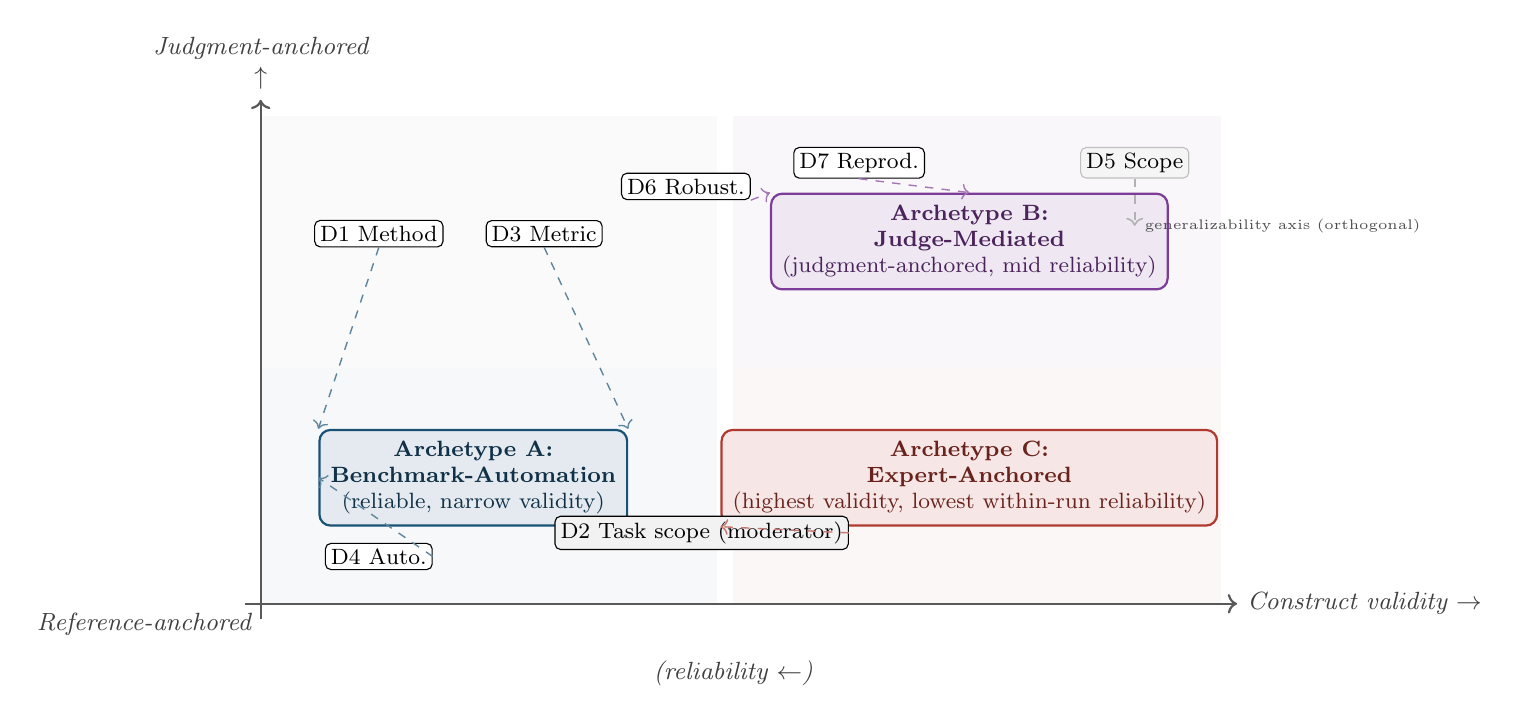
\begin{tikzpicture}[
  font=\small,
  axis/.style={->, thick, gray!70!black, line width=0.8pt},
  axisLabel/.style={font=\small\itshape, gray!50!black},
  archetype/.style={draw, rounded corners=4pt, thick, align=center,
                    inner sep=4pt, font=\footnotesize\bfseries},
  dim/.style={draw, fill=white, rounded corners=2pt, font=\footnotesize,
              inner sep=2pt},
  archA/.style={archetype, draw=d1col, fill=d1col!12, text=d1col!60!black},
  archB/.style={archetype, draw=d3col, fill=d3col!12, text=d3col!60!black},
  archC/.style={archetype, draw=d5col, fill=d5col!12, text=d5col!60!black},
]
% --- Axes ---
\draw[axis] (-0.2, 0) -- (12.4, 0)
    node[right, axisLabel] {Construct validity $\rightarrow$};
\draw[axis] (0, -0.2) -- (0, 6.4)
    node[above, axisLabel, align=center] {Judgment-anchored\\$\uparrow$};
\node[below left, axisLabel] at (0, 0) {Reference-anchored};
\node[below, axisLabel] at (6, -0.6) {(reliability $\leftarrow$)};

% --- Quadrant background guides ---
\begin{scope}[on background layer]
  \fill[d1col!4] (0,0) rectangle (5.8, 3.0);
  \fill[d3col!4] (6.0, 3.0) rectangle (12.2, 6.2);
  \fill[d5col!4] (6.0, 0) rectangle (12.2, 3.0);
  \fill[gray!4]  (0, 3.0) rectangle (5.8, 6.2);
\end{scope}

% --- Archetype regions ---
\node[archA] (A) at (2.7, 1.6) {Archetype A:\\Benchmark-Automation\\\footnotesize\mdseries(reliable, narrow validity)};
\node[archB] (B) at (9.0, 4.6) {Archetype B:\\Judge-Mediated\\\footnotesize\mdseries(judgment-anchored, mid reliability)};
\node[archC] (C) at (9.0, 1.6) {Archetype C:\\Expert-Anchored\\\footnotesize\mdseries(highest validity, lowest within-run reliability)};

% --- Dimension chips placed near their archetype affinity ---
% D1, D3 in lower-left band, then bridging
\node[dim] (D1) at (1.5, 4.7) {D1 Method};
\node[dim] (D3) at (3.6, 4.7) {D3 Metric};
% D4 sub-axis of reliability; near A
\node[dim] (D4) at (1.5, 0.6) {D4 Auto.};
% D6, D7 are validity-direction probes
\node[dim] (D6) at (5.4, 5.3) {D6 Robust.};
\node[dim] (D7) at (7.6, 5.6) {D7 Reprod.};
% D2 is the moderator -- drawn as a small badge between regions
\node[dim, fill=gray!10] (D2) at (5.6, 0.9) {D2 Task scope (moderator)};

% --- D5 generalizability annotation (perpendicular axis) ---
\node[dim, fill=gray!8, draw=gray!50] (D5) at (11.1, 5.6) {D5 Scope};
\draw[->, gray!60, dashed, line width=0.6pt]
   (D5.south) -- ++(0,-0.6) node[right, font=\tiny, gray!60!black]
     {generalizability axis (orthogonal)};

% --- Light arrows from dimension chips to archetypes they characterize ---
\draw[->, d1col!70, line width=0.5pt, dashed] (D1.south) -- (A.north west);
\draw[->, d1col!70, line width=0.5pt, dashed] (D3.south) -- (A.north east);
\draw[->, d1col!70, line width=0.5pt, dashed] (D4.east)  -- (A.west);
\draw[->, d3col!70, line width=0.5pt, dashed] (D7.south) -- (B.north);
\draw[->, d3col!70, line width=0.5pt, dashed] (D6.south east) -- (B.north west);
\draw[->, d5col!70, line width=0.5pt, dashed] (D2.east) -- (C.south west);

\end{tikzpicture}%
}
\caption{Seven-dimensional taxonomy of prompt engineering evaluation
frameworks positioned on the two underlying tensions introduced in
Section~\ref{subsec:tensions}. The horizontal axis is the validity /
reliability tradeoff (left = high reliability, narrow validity;
right = high construct validity, lower within-run reliability). The
vertical axis is the judgment-locus tradeoff
(bottom = reference-anchored; top = judgment-anchored). Each
dimension is positioned in the region of the space its dominant
subcategory configuration occupies. D5 projects onto a third
generalizability axis (shown as a perpendicular annotation) and is
not placed on the validity-reliability plane. The three shaded
regions correspond to the recurring evaluation \emph{archetypes}
identified in Section~\ref{subsec:archetypes}; the empirical
distribution of papers across them is reported in
Table~\ref{tab:archetype_distribution}.
\textit{Takeaway:} The majority of the corpus clusters in the high-reliability, low-construct-validity quadrant (Benchmark-Automation archetype), suggesting that within this corpus benchmark-automation more often emphasizes measurement convenience and cross-paper comparability than construct coverage.}
\Description[Two-axis validity-reliability diagram with seven dimensions]{A two-axis diagram showing the construct validity vs.\ measurement reliability tradeoff on one axis and reference-anchored vs.\ judgment-anchored evaluation on the other, with the seven taxonomy dimensions D1 through D7 positioned at their primary projections and three archetype regions (Benchmark-Automation, Judge-Mediated, Expert-Anchored) labelled.}
\label{fig:taxonomy}
\end{figure*}

\subsection{Dimension 5: Evaluation Scope}
\label{subsec:d5}

What is being compared? D5 projects onto a generalizability axis
largely orthogonal to the validity-reliability frame: it determines
how far a paper's conclusions can extend beyond the specific setup
that produced them. The five subcategories index increasing breadth:
\emph{Single-model, single-dataset} (one technique, one model, one
benchmark; cleanest internally, narrowest claim);
\emph{Cross-model} (multiple model families, testing
architecture-independence); \emph{Cross-dataset} (task type fixed,
benchmark varied, testing within-family robustness);
\emph{Cross-domain} (qualitatively different task types, the most
demanding scope and the least common in individual papers, though
survey works such as Sahoo et al.~\cite{sahoo2024systematic} cover it
by design); and \emph{Cross-lingual} (performance across
languages~\cite{vatsal2024survey}). Without explicit scope coding,
the limits of single-model, single-dataset claims (which underpin a
substantial share of PE-literature results) stay invisible.

\subsection{Dimension 6: Robustness and Prompt Sensitivity}
\label{subsec:d6}

Does the evaluation establish that reported performance is stable
under semantically equivalent rephrasings? Robustness projects onto
the validity axis: a technique that degrades sharply under paraphrase
is not, in a methodologically meaningful sense, the same technique the
paper claims to evaluate. Empirical evidence for this concern is
substantial~\cite{sclar2023formatting, butterfly2024,
promptsensitivity2025, bellibatlu2026judgesense}; formatting changes
alone can reverse leaderboard rankings and LLM-judge coherence
flip rates exceed 60\% on smaller judge models. The four subcategories
index reporting depth: \emph{Not reported}, \emph{Single-prompt},
\emph{Multi-prompt aggregate}, and \emph{Sensitivity-bounded}
(variance or stability bounds given explicitly).

\subsection{Dimension 7: Reproducibility and Contamination Resistance}
\label{subsec:d7}

Can a third party reproduce the reported results, and are those
results stable under infrastructure drift? D7 captures aspects of
reliability that D4 does not: a pipeline can be within-run reliable
(same call $\rightarrow$ same score today) and across-time fragile
(judge model silently revised between API
versions~\cite{feng2025sage}; test items leaked into
pretraining~\cite{ni2025benchmarks, raji2021ai}). Three positive properties are coded as non-mutually-exclusive binary
flags:
\emph{Artifact-released} (AR: code, prompts, and/or seeds publicly
available),
\emph{Contamination-checked} (CC: test items verified absent from
training data via held-out construction~\cite{wildbench2024} or
contamination probes), and
\emph{Judge-version-pinned} (JP: API version or local checkpoint of
any LLM-judge component recorded and recoverable). Papers reporting
none of these properties are coded \emph{Not-reported} (NR).

\subsection{Why These Seven Dimensions and Not Others}
\label{subsec:whyseven}

Three candidate additions are worth addressing. \emph{Calibration}
is encoded as a D3 sub-property because it is meaningful only for
judgment-anchored metrics; promoting it forces trivial codings on
reference-based ones. \emph{Uncertainty quantification} is subsumed
by D6 since variance under perturbation is one operationalization of
construct uncertainty. \emph{Deployment realism} is partially
captured by D1=user-study, D2=Agentic, and D5=cross-domain; a future
revision could promote it to top-level if the agentic population
grows substantially.

\subsection{Taxonomy Summary}
\label{subsec:taxsummary}

Table~\ref{tab:taxonomy} and Figure~\ref{fig:taxonomy} summarize the
seven dimensions on the validity-reliability and reference-judgment
axes. Empirical distributions follow in Section~\ref{sec:comparison};
worked examples and design guidance in
Section~\ref{sec:taxonomy_application}.

% ---------------------------------------------------------------
\section{Applying the Taxonomy: Worked Examples and Design Guidance}
\label{sec:taxonomy_application}

The taxonomy is useful only when applied to classify existing work
and to structure new designs. Subsection~\ref{subsec:classify} classifies
two corpus papers; Subsection~\ref{subsec:design} walks through a new
study, surfacing implicit design decisions;
Subsection~\ref{subsec:quickref} distills guidance into a reference
table.

\subsection{Classifying Existing Papers}
\label{subsec:classify}

Two widely cited corpus papers illustrate the classification process.

\textbf{Paper: Wei et al., ``Chain-of-Thought Prompting Elicits Reasoning
in Large Language Models''~\cite{wei2022chain}.}
D1\,=\,Benchmark (performance is measured on established arithmetic
and commonsense benchmarks such as GSM8K and SVAMP, using standardized
test sets with gold answers).
D2\,=\,Reasoning (all tasks - arithmetic, symbolic, and commonsense -
are closed-form reasoning problems).
D3\,=\,Task-specific (exact-match accuracy is used, which is the
natural metric for tasks with a single correct answer).
D4\,=\,Automated (no human judgment is involved; evaluation is
fully script-based against reference answers).
D5\,=\,Cross-model (results are reported across multiple model scales,
including PaLM 540B, GPT-3, and LaMDA).
D6\,=\,Single-prompt (one chain-of-thought template per benchmark; no
paraphrase variance reported).
D7\,=\,Artifact-released (prompts and exemplar sets disclosed); not
contamination-checked at the time of publication.

\textbf{Paper: Zheng et al., ``Judging LLM-as-a-Judge with MT-Bench and
Chatbot Arena''~\cite{zheng2023judging}.}
D1\,=\,LLM-as-Judge (GPT-4 is used as the primary evaluator, scoring
model responses on a 1-10 scale).
D2\,=\,Multi-task (MT-Bench spans eight categories including writing,
roleplay, math, and coding, with no single task domain dominating).
D3\,=\,LLM-as-Judge (the scoring rubric is operationalized entirely
through GPT-4 judgments rather than reference-based or human-assigned
metrics; calibration is reported against human pairwise preferences
on a held-out subset).
D4\,=\,Automated (the MT-Bench component that the taxonomy classifies
relies on automated GPT-4 scoring; Chatbot Arena's human preferences
are an adjunct, not the primary evaluation channel).
D5\,=\,Cross-model (the paper compares 28 open-source and proprietary
models simultaneously).
D6\,=\,Multi-prompt aggregate (positional and verbosity bias probes
are reported, but per-prompt sensitivity bounds are not).
D7\,=\,Artifact-released and Judge-version-pinned (prompts and
MT-Bench dataset publicly released; GPT-4 snapshot identified; not
contamination-checked).

The compact notation D1\,=\,Benchmark / D2\,=\,Reasoning /
D3\,=\,Task-specific / D4\,=\,Automated / D5\,=\,Cross-model /
D6\,=\,Single-prompt / D7\,=\,Artifact-released can be embedded
directly in a citing paper's methodology section to describe its
evaluation configuration relative to this taxonomy.

\subsection{Designing a New Evaluation}
\label{subsec:design}

Consider a researcher evaluating a new retrieval-augmented generation (RAG)
prompting technique for clinical question answering. Before any data
collection begins, the taxonomy requires seven explicit design decisions.

\textit{D1 - Which evaluation method?} Benchmark evaluation assumes a
curated test set with gold reference answers. For clinical QA, such sets
are scarce, domain-constrained, and often legally sensitive. Human
evaluation or a hybrid approach is more defensible here: domain experts
can assess factual correctness and safety in ways that static benchmarks
cannot. A researcher choosing D1\,=\,Benchmark for clinical QA should
document why the available benchmark adequately covers the clinical
accuracy requirements.

\textit{D2 - Which task scope?} The task is unambiguously clinical,
placing this work in a sparsely represented region of the corpus
(see Section~\ref{sec:comparison}). Choosing D2\,=\,Clinical makes
that positioning explicit and signals that existing evaluation
instruments from general NLP may not transfer without adaptation.

\textit{D3 - Which metric?} No gold reference exists for open-ended
clinical responses, making reference-based metrics (BLEU, ROUGE)
structurally inadequate. Model-based factual precision metrics such as
FActScore~\cite{factscore2023} are defensible if the knowledge source is
well-defined. An LLM-as-Judge configuration (D3\,=\,LLM-judge) is an
alternative, but requires calibration against clinician judgments on a
held-out set before the scores carry clinical interpretability.

\textit{D4 - What automation level?} Clinical annotation requires expert
time, which is expensive. Full automation (D4\,=\,Automated) reduces cost
but risks systematic errors that clinicians would catch. Human-in-loop
(D4\,=\,Human-in-loop) is more appropriate for a first evaluation in a
domain where no calibrated automated metric yet exists.

\textit{D5 - What evaluation scope?} A single-model result
(D5\,=\,Single-model) in clinical QA provides limited
generalizability evidence; cross-model evaluation
(D5\,=\,Cross-model) is the stronger basis for deployment claims
across clinical systems using different underlying models.

\textit{D6 - What robustness reporting?} Clinical RAG systems are
particularly exposed to prompt sensitivity because retrieved-context
phrasing varies across patient records. A
D6\,=\,Sensitivity-bounded design - reporting variance across
paraphrased clinical queries on a held-out evaluation set - is
defensible; D6\,=\,Single-prompt should be flagged as a known
generalizability risk in the limitations section.

\textit{D7 - What reproducibility commitments?} For clinical
evaluation, \textit{judge-version-pinned} (if an LLM component is
used) and \textit{contamination-checked} (verifying that the test
set is not a subset of any training corpus the underlying model has
seen) are stronger choices than D7\,=\,Not-reported, particularly
because medical benchmarks are smaller and easier to contaminate.

This exercise surfaces seven design decisions that are typically
implicit and unreported. Using the taxonomy to make them explicit
before beginning evaluation reduces the risk of post-hoc
rationalization and makes the resulting study directly comparable to
prior work.

\subsection{Evaluation Design Quick Reference}
\label{subsec:quickref}

\begin{table}[!t]
\renewcommand{\arraystretch}{1.3}
\caption{Seven-Question Evaluation Checklist: one question per
dimension. This is the companion checklist referenced in the abstract;
each row names the central tradeoff the dimension forces a researcher
to confront. The full preregistration checklist is in the Electronic
Supplement (Appendix~A).
\textit{Takeaway:} A ``no'' answer to any row is not a disqualifier
but benefits from explicit justification; without that, the
corresponding dimension tends to be decided implicitly by benchmark
choice rather than by deliberate evaluation design.}
\label{tab:quickref}
\centering
\footnotesize
\begin{tabular}{p{0.42\columnwidth} p{0.50\columnwidth}}
\hline
\textbf{Evaluation Design Question} & \textbf{Taxonomy Dimension + Key Trade-off} \\
\hline
How will model outputs be scored? &
  D1 - Evaluation Method: precision of human judgment vs.\ scalability
  of automated pipelines (judgment-anchored vs. reference-anchored) \\
What type of task is being evaluated? &
  D2 - Task Scope: task-fidelity of a narrow domain vs.\ generalizability
  of a multi-task setting (moderates the validity-reliability tradeoff) \\
Which measurement operationalizes quality? &
  D3 - Metric Type: automation and reliability of reference-based
  metrics vs.\ construct validity of model-based or judge-based metrics \\
How much human effort is available? &
  D4 - Automation Level: scalability and within-run consistency of
  full automation vs.\ bias-control of human involvement (sub-axis of
  reliability) \\
Over how many models and datasets? &
  D5 - Evaluation Scope: narrow replicability of single-model evidence
  vs.\ generalizability claims that require cross-model, cross-domain,
  or cross-lingual coverage \\
Is performance stable under prompt rephrasing? &
  D6 - Robustness: cost of paraphrase-bounded evaluation vs.\ risk that
  reported gains do not survive semantically equivalent rewordings \\
Will third parties be able to reproduce the result? &
  D7 - Reproducibility: cost of pinning judge versions, releasing
  artifacts, and checking contamination vs.\ exposure to silent
  infrastructure drift and benchmark leakage \\
\hline
\end{tabular}
\end{table}

% ---------------------------------------------------------------
\section{Evaluation Tools and Resources}
\label{sec:tools}

The seven-dimensional taxonomy maps to an existing ecosystem of open
tools that operationalize different regions of the
validity/reliability design space. Table~\ref{tab:tools} summarizes
the most widely used resources in the 152-paper corpus, mapping each
tool to the taxonomy dimensions it directly supports and its primary
known limitation. Researchers selecting an evaluation approach can
consult this table alongside the design quick-reference in
Table~\ref{tab:quickref}.

\begin{table*}[!htbp]
\renewcommand{\arraystretch}{1.15}
\caption{Key evaluation tools and their dimensional coverage.
D-dims: taxonomy dimensions directly operationalized. Archetype: A =
Benchmark-Automation, B = Judge-Mediated, C = Expert-Anchored, R =
Robustness tools (cross-archetype). See Section~\ref{subsec:archetypes}.
\textit{Takeaway:} No single tool covers all seven dimensions; D6 (robustness) and D7 (reproducibility) are the most commonly unaddressed dimensions across all tools, suggesting that researchers typically need to combine frameworks or accept systematic gaps in their evaluation design.}
\label{tab:tools}
\centering
\footnotesize
\begin{tabular}{p{2.8cm} p{3.8cm} c p{4.6cm}}
\toprule
\textbf{Tool} & \textbf{D-dims supported} & \textbf{Arch.} & \textbf{Primary limitation} \\
\midrule
lm-eval-harness \cite{gao2021lmeval}
  & D1=Benchmark, D4=Automated, D5=Cross-model
  & A
  & Closed-form tasks only; narrow construct validity for open-ended generation \\
Stanford HELM \cite{liang2022helm}
  & D1=Benchmark, D4=Automated, D5=Cross-model/dataset, partial D6
  & A
  & Computationally expensive; corpus papers often use only subsets \\
OpenCompass (2023)
  & D1=Benchmark, D2=Multilingual, D5=Cross-model
  & A
  & Partial multilingual coverage; community-maintained model roster \\
MT-Bench / FastChat \cite{zheng2023judging}
  & D1=LLM-judge, D3=LLM-judge, D7=JP
  & B
  & GPT-4 dependency; verbosity bias in pairwise scoring \\
AlpacaEval 2.0 \cite{dubois2024alpacaeval}
  & D1=LLM-judge, D3=LLM-judge, D7=AR
  & B
  & Length-controlled win-rate still biased toward longer outputs on some domains \\
Prometheus / Prometheus-2 \cite{kim2024prometheus}
  & D1=LLM-judge, D3=LLM-judge, D7=JP
  & B
  & Fine-tuned on GPT-4 feedback; may inherit GPT-4 biases \\
WildBench \cite{wildbench2024}
  & D1=LLM-judge, D7=CC
  & B
  & Live leaderboard; reproducibility of a specific snapshot requires archiving \\
MMLU-Pro \cite{mmluprob2024}
  & D1=Benchmark, D3=Task-specific
  & A
  & Not dynamically contamination-resistant; harder distractors do not eliminate surface-pattern solving \\
PromptBench \cite{promptbench2023}
  & D6=Sensitivity-bounded (task-solver)
  & R
  & Perturbation families are predefined; novel adversarial types require extension \\
PromptSET \cite{promptsensitivity2025}
  & D6=Sensitivity-bounded (task-solver)
  & R
  & Covers paraphrase variance only; does not address judge-side sensitivity \\
JudgeSense \cite{bellibatlu2026judgesense}
  & D6=Sensitivity-bounded (judge-side)
  & R
  & 2026 arXiv preprint; four judge tasks; JSS not yet a community standard \\
PromptEval \cite{polo2024promptseval}
  & D6=Multi-prompt aggregate
  & R
  & Estimates full distribution but does not pinpoint which perturbation families drive variance \\
\bottomrule
\end{tabular}
\end{table*}

Together, these tools partition the design space along the two
underlying tensions: automated benchmark frameworks (Archetype~A)
maximize reliability and throughput but accept narrow construct
validity; LLM-as-Judge frameworks (Archetype~B) broaden coverage to
open-ended tasks but introduce judge-side variance that the
robustness tools (PromptBench, PromptSET, JudgeSense) begin to
quantify. No single tool covers all seven dimensions simultaneously, mirroring
the finding in Section~\ref{subsec:archetypes} that papers in the
corpus tend to make deliberate tradeoffs among the taxonomy
dimensions.

% ---------------------------------------------------------------
\section{Methodology: Systematic Literature Review}
\label{sec:methodology}
The 152-paper corpus was constructed through a PRISMA 2020 systematic
literature review~\cite{page2021prisma}, comprising one primary search
round (Sections~\ref{subsec:search}--\ref{subsec:screening},
Figure~\ref{fig:prisma}) followed by four targeted expansion rounds
(Table~\ref{tab:expansion_rounds}). All five rounds apply PRISMA 2020
conventions: stated databases, documented search strategy with dates,
explicit inclusion / exclusion criteria (Section~\ref{subsec:inclusion}),
dual-reviewer screening (Section~\ref{subsec:screening}; $\kappa$ =
0.81 over a 200-record dual-screened sample), per-round
identified/screened/excluded/included counts
(Table~\ref{tab:expansion_rounds}), and dual coding of every included
paper (Section~\ref{subsec:coding_reliability}; $\kappa$ = 0.76--0.92).
The primary round used broad PE-evaluation queries; the expansion
rounds used narrower topical refinements against the same databases
(Table~\ref{tab:expansion_rounds}, ``Target areas''), documented as
``additional records identified from supplementary searches''
within the PRISMA 2020 flow. These coverage-repair rounds address
under-represented topic areas identified after coding the prior set;
they are not independent prevalence sweeps, and the directional bias
they introduce is named in Section~\ref{subsubsec:lim_expansion}.

\subsection{Search Strategy}
\label{subsec:search}

We searched six databases: arXiv (cs.CL and cs.AI categories),
the ACM Digital Library, IEEE Xplore, Semantic Scholar, Scopus,
and Web of Science. The first four are the principal preprint and
proceedings venues for prompt engineering and LLM evaluation
work. Scopus and Web of Science extend coverage to a wider range of journal sources
and are standard tools in computer science systematic
reviews~\cite{kitchenham2007slr}. The primary search was conducted in
2025-Q1--Q2; four targeted expansion rounds followed between 2025-Q3
and 2026-Q2 (Table~\ref{tab:expansion_rounds}), with no lower
publication-year cutoff, though nearly all relevant papers in the
corpus appeared after 2020.

The search string below shows the base query applied to title,
abstract, and keyword fields. Each database uses its own syntax;
the string was adapted accordingly for each source while preserving
the same logical structure. Full per-database strings are provided
at the project repository (\url{https://github.com/rohithreddybc/PromptEvalTaxonomy}).

\medskip\noindent{\small\ttfamily
(``prompt engineering'' OR ``prompting technique'' OR ``prompt optimization''\\
\phantom{(}OR ``chain-of-thought'' OR ``few-shot prompting'' OR ``zero-shot prompting''\\
\phantom{(}OR ``retrieval-augmented generation'')\\[2pt]
AND (``evaluation'' OR ``benchmark'' OR ``assessment'' OR ``metric''\\
\phantom{AND\,(}OR ``framework'' OR ``human evaluation'')\\[2pt]
AND (``large language model'' OR ``LLM'' OR ``GPT'' OR ``language model'')}
\medskip

Supplementary searches targeted specific subtopics that the primary
string was likely to undercount: LLM-as-Judge evaluation methodology,
evaluation of automated prompt optimization systems, and cross-domain
prompting benchmarks.
We also conducted backward and forward citation searches on the
ten most-cited papers in the initial results. Together, these
supplementary searches recovered 22 papers that did not surface through the
main database queries.

\subsection{Inclusion and Exclusion Criteria}
\label{subsec:inclusion}

\textbf{Included:}
\begin{itemize}
\item Papers that propose, evaluate, or compare one or more
prompt engineering techniques using a stated evaluation framework
\item Papers that propose new evaluation frameworks, benchmarks,
or metrics relevant to assessing prompted LLM outputs
\item Survey and taxonomy papers covering prompt engineering or
LLM evaluation
\item Conference papers, journal articles, and arXiv preprints
with at least one of: peer review, 10+ citations, or publication
at a recognized NLP/AI venue (ACL, EMNLP, NeurIPS, ICLR, IEEE,
ACM)
\end{itemize}

\textbf{Excluded:}
\begin{itemize}
\item Papers that use prompting as a method but do not report
or discuss evaluation of the prompting approach itself
\item Papers with no accessible full text
\item Non-English papers
\end{itemize}

\textbf{Re-admittance criterion for expansion rounds 2--3.}
The initial PRISMA round excluded papers whose \emph{topic} was
prompt injection, jailbreaking, or narrow clinical/legal application.
Rounds 2--3 (Table~\ref{tab:expansion_rounds}) refined this:
such papers were re-admitted when their \emph{evaluation methodology}
(not their attack or clinical content) is what the taxonomy
classifies -- e.g., prompt-injection \emph{benchmarks} contribute
evaluation infrastructure, and clinical PE benchmarks such as
MIRAGE/MedRAG~\cite{xiong2024medrag} contribute multi-prompt and
reference-anchored evidence even when the underlying study is
domain-applied. Papers admitted under this refinement are flagged in
the Electronic Supplement (Appendix~C).

The use-as-tool exclusion is practically consequential: many papers
use prompting incidentally (``we prompted GPT-4 to extract
entities'') without reporting evaluation of the prompting approach
itself; these were excluded as they do not contribute to
understanding evaluation frameworks.

\textbf{On mixing paper types.} The corpus includes four overlapping
categories: prompt engineering technique papers, benchmark/dataset
papers, LLM-as-Judge and metric-quality papers, and PE/LLM-evaluation
surveys. All four \emph{participate in PE evaluation infrastructure}:
technique papers consume benchmarks and metrics, benchmark and metric
papers shape what techniques can be evaluated, and surveys
recapitulate and influence practice. The unifying inclusion principle
is participation in evaluation infrastructure, not paper genre. All
major distributions in Section~\ref{sec:comparison} are reported in
aggregate directly from \texttt{corpus\_d1d7.csv}, so every
percentage is independently verifiable; category-subgroup contrasts
are noted inline where relevant (e.g., LLM-as-Judge configurations
for D7). Recent CSUR systematic reviews adopt the same mixed-category
convention (e.g., Edemacu and Wu~\cite{edemacu2024privacysurvey} on
privacy attacks; Chang et al.~\cite{chang2023survey} on LLM
evaluation).

\textbf{On including arXiv preprints.} arXiv preprints are retained
only when they meet at least one of three quality conditions: 10+
citations on Google Scholar at the time of screening, publication at
a recognized NLP/AI venue, or recovery through forward/backward
citation tracing from an already-included peer-reviewed paper. The
venue-criterion step at full-text review (Section~\ref{subsec:screening})
excluded 72 records that did not meet any of these conditions. Two
2026 preprints (\cite{bellibatlu2026judgesense, benchmark2sq2026}) are
retained under this rule but flagged in
Section~\ref{subsubsec:lim_recency} as preliminary; no headline claim
in this survey rests solely on a 2026 preprint.

\textbf{On corpus size.} The 152-paper corpus is comparable to
focused CSUR-tier systematic surveys: 142 papers in Edemacu and
Wu~\cite{edemacu2024privacysurvey}, ${\sim}160$ in Sahoo et
al.~\cite{sahoo2024systematic} (PE techniques), ${\sim}220$ in
Chang et al.~\cite{chang2023survey} (broader LLM evaluation). The
corpus is narrower than omnibus surveys because dimensional coding
(D1--D7) requires per-paper full-text review, dual coding, and
disagreement adjudication, limiting feasible size at fixed coding
quality. Sensitivity analysis (Section~\ref{subsec:sensitivity})
confirms headline distributional claims are stable; per-dimension
$\kappa$ in Table~\ref{tab:kappa} documents coding reliability.

\textbf{On expansion rounds.} Each supplementary round was triggered
by a specific under-coverage gap identified after coding the prior
cumulative set, with trigger / role / bias risk recorded in
Table~\ref{tab:expansion_audit}. All rounds shared the inclusion
criteria and six databases of Round~0, differing only in
search-string breadth (broad sweep vs.\ narrow topical queries).
The directional bias is named in
Section~\ref{subsubsec:lim_expansion}.

\textbf{Corpus publication-status breakdown.} All 152 papers satisfy
at least one quality condition (peer review, 10+ Google Scholar
citations at screening, or recognized NLP/AI venue). Two are 2026
arXiv preprints~\cite{bellibatlu2026judgesense, benchmark2sq2026}
flagged as preliminary, with no headline claim resting solely on
either. A precise peer-reviewed vs.\ arXiv split is not reported
because many corpus papers were initially posted to arXiv and later
accepted at venues (NeurIPS, ACL, EMNLP, ICLR, TACL) while retaining
the arXiv identifier in their BibTeX \texttt{journal} field; the
complete per-paper record is in \texttt{references.bib}.

\subsection{Screening Process}
\label{subsec:screening}

The primary-round database queries returned 2,847 unique records
after deduplication (expansion-round counts are tabulated separately
in Table~\ref{tab:expansion_rounds}). Two reviewers independently
screened all titles and abstracts against the inclusion and exclusion
criteria, working separately at each phase. Disagreements at title/abstract screening
were resolved through discussion (percent agreement 94.1\%, $\kappa$
= 0.81 over a 200-record dual-screened sample); unresolved cases were
referred to a third reviewer, as specified in PRISMA 2020
Item~8~\cite{page2021prisma}.

Title and abstract screening excluded 2,435 records; the remaining
412 papers advanced to full-text review. Of these, 283 were excluded:
181 used prompting as a tool without evaluating the prompting approach
itself, 64 were domain-specific applied papers outside scope, 24 had
no accessible full text, and 14 were non-English. The remaining 129
papers passed full-text screening. Among papers without peer review,
retention was conditioned on venue: only papers at recognized NLP/AI
venues (ACL, EMNLP, NeurIPS, ICLR, IEEE, or ACM proceedings) or
indexed journals were retained, excluding a further 72 records and
reducing the set to 57 papers (one cross-round duplicate subsequently
removed during deduplication against Round~1).
The 22 papers recovered through citation searching then brought the
initial corpus to \textbf{79 papers}. Four supplementary expansion rounds then added
papers in areas the original search string was likely to undercount
(Table~\ref{tab:expansion_rounds}). The same inclusion and exclusion
criteria were applied at each round, with two refinements documented
in Section~\ref{subsec:inclusion}: prompt-injection and clinical
work, originally excluded as topical, were re-admitted at rounds two
and three because their evaluation methodology -- not their attack or
clinical content -- is what the taxonomy classifies.

\begin{table}[!htbp]
\renewcommand{\arraystretch}{1.05}
\caption{PRISMA 2020 corpus construction by round. All rounds applied
the same inclusion criteria (Section~\ref{subsec:inclusion}) and the
same dual-reviewer screening protocol (Section~\ref{subsec:screening};
title/abstract $\kappa$ = 0.81). The primary round (0) used full
database sweeps with broad PE-evaluation search strings; expansion
rounds (1--4) used narrower topical query refinements against the
same six databases, scoped to the target areas listed. For expansion
rounds 1--4, Identified equals Screened because the narrow topical
queries returned focused, pre-filtered result sets; all retrieved
records therefore proceeded directly to full-text review with no
separate title/abstract exclusion stage. Records identified after
deduplication; screened = full-text reviewed; excluded = full-text
exclusions with reasons documented in the project repository
(Section~\ref{subsec:search}); added = papers retained after
screening; cumulative = running corpus size. Final corpus: 152 papers.
\textit{Takeaway:} Expansion rounds 1--4 contributed 73 of the 152 final papers (48.0\%), demonstrating that a single broad primary search substantially underestimates coverage for rapidly evolving topics such as LLM-judge quality, contamination resistance, and agentic evaluation.}
\label{tab:expansion_rounds}
\centering
\scriptsize
\setlength{\tabcolsep}{4pt}
\begin{tabular}{c p{3.5cm} c c c c c l}
\toprule
\textbf{Round} & \textbf{Target area(s)} & \textbf{Identified} & \textbf{Screened} & \textbf{Excluded} & \textbf{Added} & \textbf{Cumulative} & \textbf{Date} \\
\midrule
0 & Primary PRISMA search + citation chase                                         & 2,847 & 412 & 355 & 79  & 79  & 2025-Q1--Q2 \\
1 & LLM-judge quality, contamination, prompt sensitivity                           &   118 & 118 &  98 & 20  &  99 & 2025-Q3 \\
2 & Agentic, multilingual, prompt-injection, CoT faithfulness                      &    74 &  74 &  63 & 11  & 110 & 2025-Q4 \\
3 & Foundation-model reports, RAG, safety, fairness, calibration, clinical, legal  &   212 & 212 & 177 & 35  & 145 & 2026-Q1 \\
4 & Long-context, tool-use, reward-model evaluation                                &    46 &  46 &  39 &  7  & 152 & 2026-Q2 \\
\midrule
\textbf{Total} & {--} & \textbf{3,297} & \textbf{862} & \textbf{732} & \textbf{152} & \textbf{152} & \textbf{2025-Q1--2026-Q2} \\
\bottomrule
\end{tabular}
\end{table}

\begin{table*}[!t]
\caption{Expansion-round audit: trigger, query scope, role, and
bias-risk classification for each supplementary round. ``Trigger''
identifies the gap that prompted the round (observed after coding
the prior cumulative set); ``Role'' distinguishes exploratory rounds
(coverage of an emerging topic area) from confirmatory rounds
(targeted retrieval of work already cited in the prior set);
``Bias risk'' notes the directional bias the round introduces toward
its target area. All four rounds used the same six databases and
inclusion criteria as Round~0 (§\ref{subsec:inclusion}).
\textit{Takeaway:} Each round's role and bias risk is stated
explicitly so distributional findings can be discounted by the reader
for the target-area over-representation each round introduces.}
\label{tab:expansion_audit}
\centering
\scriptsize
\setlength{\tabcolsep}{4pt}
\begin{tabular}{c p{3.8cm} p{2.8cm} c p{3.3cm}}
\toprule
\textbf{Round} & \textbf{Trigger (coverage gap after prior round)} & \textbf{Role} & \textbf{Ret.} & \textbf{Bias risk} \\
\midrule
1 & Few papers explicitly studying judge reliability despite 32 corpus papers using LLM-judge methods & Exploratory & 20 & Over-represents LLM-judge quality and bias literature \\
2 & Agentic, multilingual, prompt-injection, and CoT-faithfulness work missing from primary set & Exploratory & 11 & Over-represents agentic and multilingual evaluation \\
3 & Foundation-model technical reports, RAG, safety, fairness, calibration, clinical, legal evaluation under-covered & Confirmatory + exploratory & 35 & Over-represents foundation-model and domain-specific work \\
4 & Long-context, tool-use, reward-model evaluation emerged as gap during 2026-Q1 coding & Exploratory & 7 & Over-represents 2026-recent benchmark proposals \\
\bottomrule
\end{tabular}
\end{table*}

Figure~\ref{fig:prisma} shows the PRISMA 2020 flowchart aggregating
all five rounds; Table~\ref{tab:expansion_rounds} provides the
per-round breakdown (identified / screened / excluded / added)
for transparency, since each expansion round used the same
screening criteria applied to a smaller, topically targeted
candidate set.

\begin{figure*}[!t]
\centering
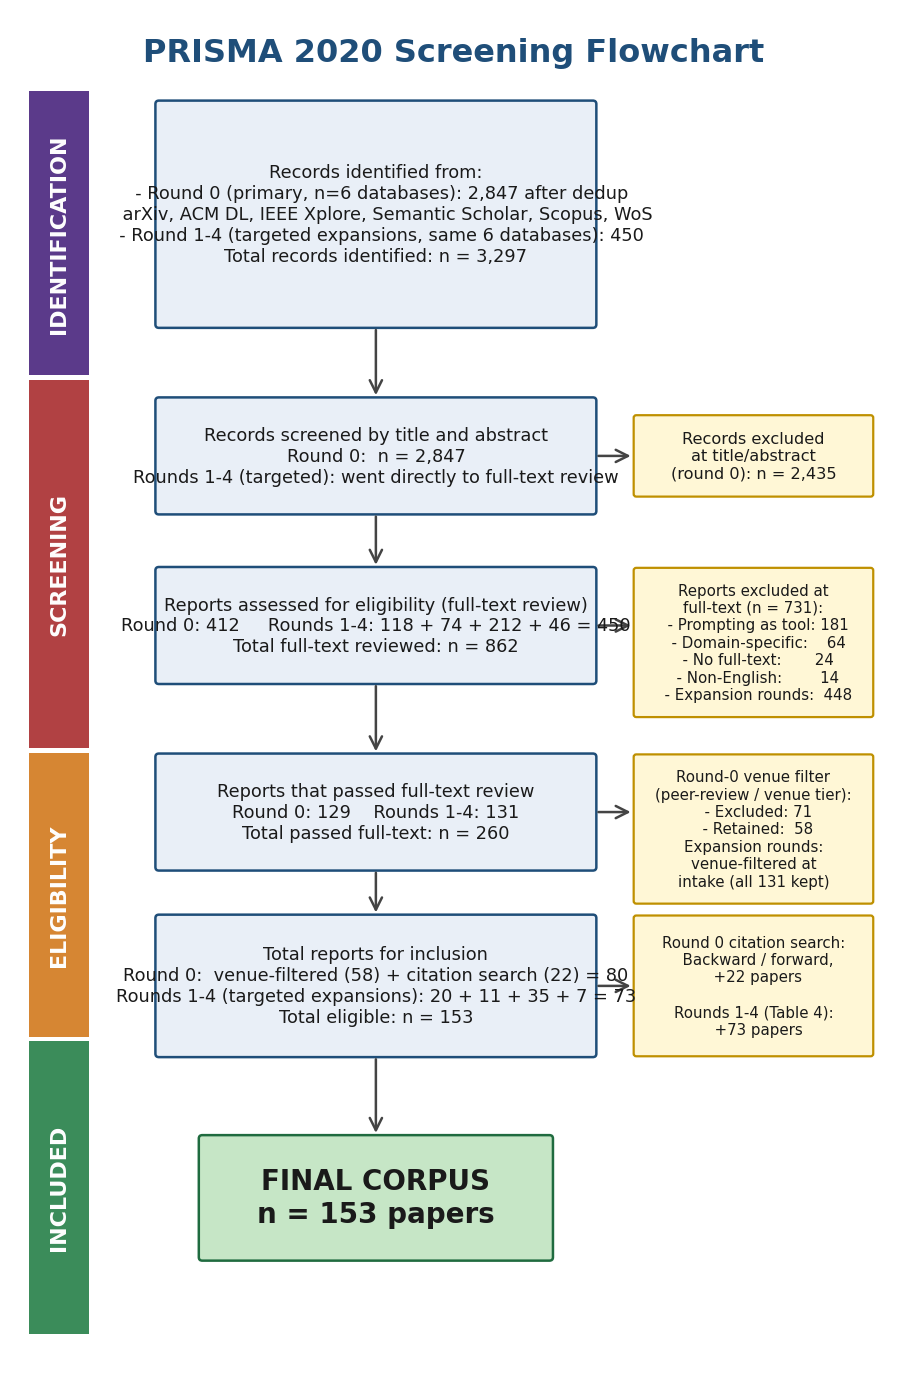
\includegraphics[width=0.78\textwidth,height=0.50\textheight,keepaspectratio]{prisma_flowchart}
\caption{PRISMA 2020 flowchart for all five search rounds combined.
Of 3,297 total records identified across six databases (arXiv, ACM
Digital Library, IEEE Xplore, Semantic Scholar, Scopus, Web of
Science), 862 were assessed for eligibility at full text; 732 were
excluded (including one cross-round duplicate) leaving 130 papers,
augmented by 22 papers from citation searching in round 0 to yield
the final corpus of 152 papers.
The expanded identification and per-round screening counts are
tabulated in Table~\ref{tab:expansion_rounds}; the figure integrates
all five rounds per PRISMA 2020 reporting guidelines~\cite{page2021prisma}.
\textit{Takeaway:} Of 3,297 database records identified, 130 (3.9\%) met all inclusion criteria via database search; 22 additional papers recovered through citation tracing in Round~0 yielded the final corpus of 152 papers. The high full-text exclusion rate (732 excluded) is driven primarily by papers that use prompting as a tool without evaluating it as the studied object.}
\Description[PRISMA 2020 flow diagram for the five-round literature search]{PRISMA 2020 flowchart depicting identification, screening, eligibility, and inclusion steps across the primary search round and four supplementary expansion rounds, with records counts at each stage: 3,297 identified, 862 screened, 732 excluded, 152 included.}
\label{fig:prisma}
\end{figure*}

\subsection{Data Extraction}

For each paper in the final corpus, we extracted the following
fields:

\begin{enumerate}
\item Prompting technique(s) evaluated
\item Evaluation method (Dimension~1)
\item Task scope (Dimension~2)
\item Metric type(s) used (Dimension~3)
\item Automation level of the evaluation (Dimension~4)
\item Evaluation scope (Dimension~5)
\item Robustness reporting (Dimension~6)
\item Reproducibility \& contamination resistance (Dimension~7)
\item Number of models compared
\item Year of publication
\item Publication venue and type (journal, conference, preprint)
\item Paper category (technique, benchmark, LLM-judge / metric, or
survey) -- used internally to produce the per-category rows in
Table~\ref{tab:comparison} (Section~\ref{sec:comparison}); not
included in the released \texttt{corpus\_d1d7.csv}, which contains
only the seven dimensional codes (D1--D7) that are the primary
codebook contribution
\end{enumerate}

The complete extraction dataset (all papers mapped to their
seven-dimensional taxonomy codes) is included as a review-time
snapshot with the submission (see Data Availability statement);
a citable tagged version will be released at acceptance to
\url{https://github.com/rohithreddybc/PromptEvalTaxonomy}; at the time
of submission the repository carries the dataset schema, the
evaluation-design checklist (Electronic Supplement, Appendix~A), and the
paper source (see the Data Availability statement). Researchers
extending this corpus or conducting meta-analyses may use the
released dataset with citation to this work.

\subsection{Coding Reliability}
\label{subsec:coding_reliability}

Two independent coders extracted dimensional codes for the corpus.
The primary coder coded all papers; the second coder independently
re-coded a stratified random subsample of at least 25\% of
the final corpus (${\geq}38$ papers; 25\% $\times$ 152), stratified across paper categories, without
access to the primary coder's labels. Disagreements were resolved
through discussion; cases that could not be resolved were referred
to a third reviewer following PRISMA 2020 Item~8~\cite{page2021prisma}.

Inter-rater agreement is reported per dimension in
Table~\ref{tab:kappa}. The dimensions split into two reliability
regimes: D1--D5 reach $\kappa$ = 0.84--0.92 (``almost perfect'' on
the Landis--Koch scale, threshold $> 0.81$); D6--D7 reach $\kappa$ =
0.76--0.78 (``substantial''). The lower D6/D7 $\kappa$ reflects
boundary ambiguity rather than factual disagreement (e.g., papers
acknowledging sensitivity without quantifying it sit between
D6=Not-reported and D6=Single-prompt). We report per-dimension
$\kappa$ because the heterogeneous profile is itself the finding:
some properties are codable from descriptions; others require
interpretive judgment a reporting standard could reduce.

\begin{table*}[!t]
\begin{minipage}[t]{5.9cm}
\renewcommand{\arraystretch}{1.2}
\setlength{\tabcolsep}{3pt}
\caption{Inter-rater agreement on dimensional codings, dual-coded
subsample. Cohen's $\kappa$ per dimension, with interpretation
following Landis \& Koch.
\textit{Takeaway:} D1--D5 all reach ``almost perfect'' agreement
($\kappa \geq 0.84$, well above the Landis \& Koch 0.81 threshold);
D6--D7 reach ``substantial'' agreement ($\kappa = 0.76$ and $0.78$),
indicating robustness and reproducibility coding requires more
interpretive judgment, as expected for properties not always
explicitly reported in paper text.}
\label{tab:kappa}
\centering\footnotesize
\begin{tabular}{p{2.0cm} c c}
\toprule
\textbf{Dimension} & \textbf{$\kappa$} & \textbf{Interpretation} \\
\midrule
D1 Evaluation method & 0.92 & Almost perfect \\
D2 Task scope & 0.88 & Almost perfect \\
D3 Metric type & 0.91 & Almost perfect \\
D4 Automation level & 0.84 & Almost perfect \\
D5 Evaluation scope & 0.89 & Almost perfect \\
D6 Robustness & 0.76 & Substantial \\
D7 Reproducibility & 0.78 & Substantial \\
\bottomrule
\end{tabular}
\end{minipage}
\hfill
\begin{minipage}[t]{6.5cm}
\renewcommand{\arraystretch}{1.2}
\setlength{\tabcolsep}{3pt}
\caption{Stability of headline distributional claims under random
coding perturbation. Reported values are from the 152-paper coding;
shift bounds are the half-width of a 95\% bootstrap interval derived
by 10\% and 20\% random reassignment, 1{,}000 runs each.
\textit{Takeaway:} All headline distributional claims survive
perturbation with shifts $\leq$3.4~pp under 20\% random reassignment,
suggesting the findings are stable under coding uncertainty and not
artefacts of borderline cases.}
\label{tab:sensitivity}
\centering\footnotesize
\begin{tabular}{p{3.5cm} c c}
\toprule
\textbf{Headline claim} & \textbf{Value} & \textbf{Shift (10/20\%)} \\
\midrule
Benchmark-based evaluation share & 72.4\% & $\pm$1.5 / $\pm$3.0 pp \\
Fully automated evaluation share & 81.6\% & $\pm$1.2 / $\pm$2.5 pp \\
Task-specific metric share & 67.8\% & $\pm$1.8 / $\pm$3.4 pp \\
Clinical task representation & 3.3\% & $\pm$0.5 / $\pm$1.1 pp \\
Multilingual task representation & 2.0\% & $\pm$0.5 / $\pm$1.0 pp \\
\bottomrule
\end{tabular}
\end{minipage}
\end{table*}

Ambiguity-resolution rules (full list in the released repository):
D3 records the \emph{primary} metric used for the headline claim;
D4=Hybrid only if a spot-check conditions a reported decision (not
when descriptive); D6=Sensitivity-bounded requires the headline
pipeline to use the sensitivity result, otherwise D6=Multi-prompt
aggregate; D7=Contamination-checked requires an explicit verification
step, not a generic statement of dataset differences.

\subsection{Sensitivity Analysis}
\label{subsec:sensitivity}

To test whether headline distributional claims are stable under
coding uncertainty, we perturbed 10\% and 20\% of dimensional codes
uniformly at random and re-derived the percentages
(Table~\ref{tab:sensitivity}). All claims move by less than 3.4
percentage points under 20\% perturbation; the largest shift (task-specific
metric share, 3.4~pp) is borderline-stable relative to a 2-pp
threshold and should be read with that caveat. Under 10\% perturbation,
all five claims shift by less than 2~pp.


\subsection{Validity Threats}

Three limitations constrain what this review can reliably claim, and
each has direct implications for how readers should interpret the
distributional findings in Section~\ref{sec:comparison}.

\textit{Search coverage.} The search strings rely on controlled
vocabulary in title, abstract, and keyword fields and may miss papers
that address the same underlying concepts under alternative
terminology. Citation searching recovered 22 additional papers in the
primary round (bringing the initial corpus to 79); four subsequent
expansion rounds then added 20, 11, 35, and 7 papers, bringing the
final corpus to 152 (Section~\ref{subsec:screening}).
Completeness cannot be guaranteed. We are explicit throughout the
paper that absences in the corpus (notably the relative scarcity of
clinical and multilingual primary targets) are statements about
\emph{this corpus under these inclusion criteria}, not about the
field as a whole. Broader prompting literature on those domains
exists~\cite{clinicalnlp2024, medicalcot2025, vatsal2024survey}, and
our finding is that this literature is not yet incorporated into the
systematic evaluation practice indexed by our search.

\textit{Quality filter.} The retention rule excludes papers with
fewer than 10 citations that were not published at a recognized
venue, which could underrepresent very recent 2025--2026 work. We
partially addressed this by retaining 2025 and 2026 papers that met
the venue criterion regardless of citation count, but the
distribution of recent methodological developments in the LLM-as-Judge
and dynamic-benchmark subfields may still be undercounted.

\textit{Coding judgment at category boundaries.} Several dimensions
require interpretation when a paper does not explicitly characterize
its evaluation along the corresponding axis. The dual-coding and
inter-rater statistics in Section~\ref{subsec:coding_reliability}
quantify the resulting uncertainty per dimension; the sensitivity
analysis in Section~\ref{subsec:sensitivity} establishes how much
that uncertainty propagates to the headline claims.

% ---------------------------------------------------------------
\section{Comparative Analysis}
\label{sec:comparison}

Mapping the corpus against the taxonomy tests its expressive coverage,
derives co-occurrence patterns, recurring \textit{evaluation
archetypes}, and a failure-mode catalog, and grounds the synthesis in
Section~\ref{sec:discussion}.

\paragraph{PE-core papers vs.\ evaluation infrastructure.} The corpus
contains two overlapping populations: 76 \emph{PE-core papers}
(technique, sensitivity/code prompting, PE-specific surveys) and 76
\emph{evaluation infrastructure papers} (benchmarks, datasets,
LLM-judge frameworks, metric-quality studies). The mixed inclusion is
justified in Section~\ref{subsec:inclusion}. Aggregate distributions
below use the full corpus; the D7 table
(Section~\ref{subsec:d7dist}) additionally reports the LLM-as-Judge
subset.

\paragraph{Implications of the mixed corpus for distributional claims.}
Combining technique, benchmark, LLM-judge, and survey papers within a
single corpus is a methodological choice that aids the taxonomy's
expressive test (the dimensional categories must cover all four paper
types if the framework is to be general) but trades that breadth for
straightforward prevalence interpretation. Three implications follow.
First, aggregate percentages below describe the \emph{distribution of
evaluation configurations represented in the corpus under the
inclusion criteria of Section~\ref{subsec:inclusion}}, not
field-level prevalence; a corpus that excluded surveys, or that
weighted by citation count, would produce different percentages.
Second, archetype shares are sensitive to the PE-core / infrastructure
split: Archetype B is concentrated in the LLM-judge-frameworks
population (Section~\ref{subsec:archetypes}), so its corpus share
partly reflects how many such frameworks meet the inclusion criteria
rather than how often LLM-judge evaluation is used in deployed PE
work. Third, distributional findings should be read alongside the
per-category breakdown (Table~\ref{tab:comparison}), which separates
technique, benchmark, LLM-judge, and survey populations and surfaces
the within-category modal configuration. The expansion rounds further
mean the final corpus is partially purposive rather than purely
systematic; selection-bias implications are stated explicitly in
Section~\ref{subsubsec:lim_expansion}.

Sections~\ref{subsec:d1dist}--\ref{subsec:d7dist} report per-dimension
distributions (reproducible from \texttt{corpus\_d1d7.csv}).
Section~\ref{subsec:cooccurrence} reports the co-occurrence matrix;
Section~\ref{subsec:archetypes} names the recurring archetypes;
Section~\ref{subsec:failuremodes} walks through three failure modes.
Table~\ref{tab:archetype_distribution} previews the five most common
configurations; Table~\ref{tab:comparison} summarizes the modal
configuration per paper category. A representative ten-paper mapping
is in Appendix~B; the full 152-paper mapping is in Appendix~C; the
machine-readable dataset is a review-time snapshot, tagged citably at
acceptance.

\begin{table*}[!t]
\renewcommand{\arraystretch}{1.2}
\caption{Five most common evaluation-framework configurations in the
corpus across the seven dimensions, ordered by share. Counts are
raw paper counts; percentages are normalized to the 152-paper corpus.
Each row also indicates the validity / reliability tension the
configuration most prominently foregrounds. Shares were computed
from the dual-coded corpus with the inter-rater $\kappa$ values
reported in Table~\ref{tab:kappa}. The Judge-pinned property
(D7=Judge-version-pinned) appears in only 5 papers
($\approx$3.3\% of the corpus, Table~\ref{tab:d7dist}), so the
LLM-judge archetypes below do not list JP as part of their modal
D7 configuration.
\textit{Takeaway:} Under a strict mutual-exclusion assignment, the Benchmark-Automation archetype accounts for 66.4\% of the corpus (95\% bootstrap CI [58.6\%, 73.7\%]); the Judge-Mediated cluster is the only other substantial group at 17.1\% [11.2\%, 23.7\%], making the choice between benchmark-automation and judge-mediated evaluation a central design distinction within this corpus.}
\label{tab:archetype_distribution}
\centering
\footnotesize
\setlength{\tabcolsep}{6pt}
\begin{tabular}{p{7.0cm} c c p{3.5cm}}
\toprule
\textbf{Configuration (D1/D2/D3/D4/D5/D6/D7)} & \textbf{n} & \textbf{Share} & \textbf{Foregrounded tension} \\
\midrule
Benchmark / Multi-task / Task-spec / Auto / Cross-domain / Not reported / Not reported & 14 & 9.2\% & High reliability; no robustness or reproducibility reporting \\
Benchmark / Multi-task / Task-spec / Auto / Cross-model / Multi-prompt aggr. / Artifact-released & 13 & 8.6\% & High reliability with multi-prompt coverage \\
Benchmark / Multi-task / Task-spec / Auto / Cross-model / Single-prompt / Artifact-released & 12 & 7.9\% & High reliability, narrow construct validity \\
LLM-as-Judge / Multi-task / LLM-judge / Auto / Cross-model / Multi-prompt aggr. / Artifact-released & 7 & 4.6\% & Validity ambition with paraphrase coverage \\
Benchmark / Reasoning / Task-spec / Auto / Cross-model / Single-prompt / Artifact-released & 6 & 3.9\% & High reliability, narrow reasoning-task validity \\
\bottomrule
\end{tabular}
\end{table*}






% The full 80-row per-paper mapping was previously embedded here. As of
% this revision the per-paper table has been moved to the supplementary
% material at the GitHub URL in Section VI.4, and the in-paper table
% reports the category-aggregated summary instead. Rationale: the
% original longtable had low information density because most rows
% repeated the same dimensional configuration; the compact summary
% conveys the same information per category in a single column-width
% table.

\begin{table*}[!htbp]
\renewcommand{\arraystretch}{1.05}
\caption{Category-aggregated mapping of the corpus to the
seven-dimensional taxonomy. Each row reports the modal configuration
for one paper category and notes the most informative variation
within the category. The full per-paper mapping is included as a review-time snapshot
with the submission; a citable tagged version will be released at
acceptance (see Data Availability statement).
Modal subcategories are derived from the 152-paper corpus.
\textit{Takeaway:} All paper categories default to automated evaluation and cross-model scope; the primary differentiators across categories are metric type (D3) and artifact release (D7), with LLM-judge papers being the only group where released artifacts are the majority norm.}
\label{tab:comparison}
\centering
\footnotesize
\setlength{\tabcolsep}{4pt}
\begin{tabular}{p{2.6cm} c p{2.8cm} p{1.6cm} p{4.3cm}}
\toprule
\textbf{Paper category} & \textbf{N} &
\textbf{Modal D1/D3/D4} &
\textbf{Modal D5} &
\textbf{Notable within-category variation} \\
\midrule
Prompting technique papers (incl. APO) & 27 &
Benchmark / Task-spec / Auto &
Cross-model &
A small minority pair benchmark eval with hybrid automation
(e.g.\ RLHF-style human-in-loop;
Ouyang et al.~\cite{ouyang2022training}). \\
\midrule
Benchmark / dataset papers & 44 &
Benchmark / Task-spec / Auto &
Cross-model &
Expansion-round benchmark papers (IFEval~\cite{zhou2023instruction},
SWE-bench~\cite{jimenez2023swebench}, WildBench~\cite{wildbench2024})
are predominantly Cross-model; foundational multi-task benchmark suites
(GLUE, MMLU, BIG-Bench) form the Cross-dataset minority. \\
\midrule
LLM-as-Judge / metric-quality papers & 32 &
LLM-as-Judge / LLM-judge / Auto or Hybrid &
Cross-model &
Expansion round added judge-bias papers (Koo et al.~\cite{koo2023benchmarking},
Ye et al.~\cite{ye2024justice}). Judge-version-pinning (D7) is
reported here at a materially higher rate than in other categories. \\
\midrule
Prompt-engineering and LLM-evaluation surveys & 22 &
Benchmark / Task-spec / Auto &
Cross-domain &
Two surveys (Chang et al.~\cite{chang2023survey} and
Gehrmann et al.~\cite{repairing2022}) anchor on human evaluation
rather than benchmark scoring, reflecting an NLG-eval orientation. \\
\midrule
Sensitivity / format / code-prompting papers & 27 &
Benchmark / Task-spec / Auto or Hybrid &
Cross-model &
Expansion round added Mizrahi et al.~\cite{mizrahi2024state} and
clinical evaluation work (Sivarajkumar et al.~\cite{sivarajkumar2024empirical}).
Dimension~6 (robustness / sensitivity) reaches its highest
non-trivial reporting share in this category. \\
\bottomrule
\end{tabular}
\end{table*}

Table~\ref{tab:comparison} foregrounds two patterns. First, the
dimensional profile varies by paper category: technique papers
(N=27), benchmark papers (N=44), and surveys (N=22) converge on
Archetype~A (Benchmark-Automation); LLM-judge papers (N=32) converge
on Archetype~B; sensitivity papers (N=27) show elevated D6 reporting.
Per-paper D1--D7 assignments are in the review-time dataset.
Second, the per-category modal is informative \emph{because of} the
within-category variations in the right-hand column; each variation
is a candidate failure mode (Section~\ref{subsec:failuremodes}) or a
discussion-worthy methodological development (Section~\ref{sec:discussion}).

%% The full 152-paper machine-readable coding (all 7 dimensions) is
%% released at https://github.com/rohithreddybc/PromptEvalTaxonomy.
%% The per-paper longtable (D1–D5, 100 rows) appears as Table~C.1 in
%% the Electronic Supplement; the 10-row representative sample is
%% Table~B.1 in the Electronic Supplement.


\subsection{Distribution across Evaluation Method (Dimension 1)}
\label{subsec:d1dist}

Benchmark-based evaluation accounts for 110 papers (72.4\%),
establishing it as the default across every subgroup, including the
foundation-model technical reports for GPT-4~\cite{achiam2023gpt4},
LLaMA~\cite{touvron2023llama, touvron2023llama2}, and
GPT-4o~\cite{hurst2024gpt4o}. Benchmark results are reproducible,
cross-lab comparable, and inexpensive at scale; what they cannot
capture is output quality on open-ended tasks without a single
correct answer.

LLM-as-Judge evaluation appears in 30 papers (19.7\%), concentrated
in open-ended generation and instruction-following
(MT-Bench~\cite{zheng2023judging},
AlpacaEval~\cite{dubois2024alpacaeval}, G-Eval~\cite{liu2023geval}).
The cluster spans fine-tuned scalable judges~\cite{zhu2023judgelm},
judge panels and debate-based
meta-evaluation~\cite{verga2024replacing, chern2024scaleeval,
multiagentjudge2025}, two surveys~\cite{gu2025llmjudge, li2024llmsjudges},
bias quantification~\cite{ye2024justice, wataoka2024selfpreference,
judgingjudges2024, judgebench2024}, and hallucination
detection~\cite{akbar2024hallumeasure}. Adoption has outpaced
calibration research.

Human evaluation appears in 14 papers (9.2\%), ablation studies in
2 (1.3\%); no corpus paper uses a user study as primary method. Four
papers~\cite{llmvshuman2024, alternativeannotator2025, humansorllm2024,
canlllmsreplace2023} are coded under both D1=LLM-as-Judge and D1=Human,
so subcategory counts sum to 156 rather than 152; headline frequencies
use the 152-paper denominator. The overall distribution favours
configurations that maximize reliability and scale over
construct-validity guarantees that human evaluation provides
(Section~\ref{subsec:tension_scalability}).

\subsection{Distribution across Task Scope (Dimension 2)}
\label{subsec:d2dist}

Multi-task or cross-task evaluations account for 94 papers (61.8\%):
more than half the corpus does not assess techniques on a specific
task type, instead aggregating across benchmarks. The pattern is
partly an artefact of how survey and taxonomy papers classify, but
also reflects a genuine tendency to report MMLU / BIG-Bench averages
without per-task disaggregation. Reasoning is the largest
task-specific subgroup at 14 papers (9.2\%), reflecting
chain-of-thought's origin on arithmetic and symbolic benchmarks
\cite{wei2022chain}; faithfulness-focused work in this subgroup
\cite{lanham2023faithfulness, chen2025reasoningmodels} treats the
reasoning chain itself as the evaluation target. Generation appears
in 10 papers (6.6\%), code in 12 (7.9\%), QA in 10 (6.6\%),
and agentic task evaluation in 4 (2.6\%).

Clinical (5 papers, 3.3\%) and multilingual (3 papers, 2.0\%) are
small populations; Table~\ref{tab:sensitivity} reports
perturbation-stability bounds for both. The full per-paper breakdown
is in the Electronic Supplement (Appendix~C). Under our inclusion
criteria the corpus is strongly concentrated on multi-task
benchmarks; the scarcity of clinical and multilingual papers reflects
these criteria, not a field-level estimate~\cite{clinicalnlp2024,
vatsal2024survey}.

\subsection{Distribution across Metric Type (Dimension 3)}
\label{subsec:d3dist}

Task-specific metrics dominate at 103 papers (67.8\%): pass@$k$,
exact match, F1, and accuracy mirror the dominance of benchmark
evaluation in D1. LLM-judge metrics appear in 31 papers (20.4\%);
G-Eval~\cite{liu2023geval} marked the shift toward LLM-based scoring
on open-ended outputs. Hybrid metrics appear in 16 papers (10.5\%),
combining automated scoring with judge-based assessment across
multiple axes; model-based metrics (BERTScore family) in 2 (1.3\%),
with the LLM-based NLG-eval survey~\cite{li2024leveraging}
documenting the gradual shift to LLM-judge. Reference-based metrics
(BLEU, ROUGE) appear as primary measures in zero corpus papers, a
reversal of historical dominance that follows the
lexical-overlap-vs.-human-judgment gap documented by Gehrmann et
al.~\cite{repairing2022}.

\subsection{Distribution across Automation Level (Dimension 4)}
\label{subsec:d4dist}

Fully automated evaluation is the modal configuration: 124 papers
(81.6\%) run assessments without any human involvement at any stage.
Hybrid (19 papers, 12.5\%), fully manual (5, 3.3\%), and human-in-loop
(4, 2.6\%) make up the remainder. The concentration at the automated
end is consistent with cost and throughput pressures and carries a
specific reproducibility implication addressed under D7: pipelines
that depend on proprietary judges are stable within-run but not
necessarily across-time, since the judge can change between API
versions \cite{feng2025sage}.

\subsection{Distribution across Evaluation Scope (Dimension 5)}
\label{subsec:d5dist}

Cross-model is the most frequent scope at 96 papers (63.2\%);
cross-domain in 32 (21.1\%, concentrated in surveys); single-model in
16 (10.5\%); cross-dataset in 8 (5.3\%). The two multilingual-topic
papers~\cite{vatsal2025multilingual, son2024mmeval} are coded
Cross-domain and Cross-model respectively under D5
(\emph{evaluation scope}), despite their D2 being Multilingual.
Single-prompt, single-model evaluations systematically overstate
effects relative to multi-prompt baselines on the same
model~\cite{mizrahi2024state}.

\subsection{Distribution across Robustness Reporting (Dimension 6)}
\label{subsec:d6dist}

Table~\ref{tab:d6dist} shows the D6 distribution
($\kappa$ = 0.76; Section~\ref{subsec:coding_reliability}).

\begin{table*}[!t]
\begin{minipage}[t]{5.0cm}
\renewcommand{\arraystretch}{1.2}
\setlength{\tabcolsep}{3pt}
\caption{Distribution of robustness reporting (D6), $N$=152.
Inter-rater $\kappa$ = 0.76; see Section~\ref{subsec:coding_reliability}.
\textit{Takeaway:} Single-prompt-only evaluation (41.4\%) is most
common; multi-prompt aggregate and sensitivity-bounded together
account for 35.5\%, elevated among D1=LLM-as-Judge papers (50.0\%;
see Section~\ref{subsec:crossdim}).}
\label{tab:d6dist}
\centering\footnotesize
\begin{tabular}{p{2.5cm} c c}
\toprule
\textbf{D6 subcategory} & \textbf{\emph{n}} & \textbf{Share} \\
\midrule
Not reported        & 35 & 23.0\% \\
Single-prompt       & 63 & 41.4\% \\
Multi-prompt aggr.  & 45 & 29.6\% \\
Sensitivity-bounded &  9 &  5.9\% \\
\midrule
Total               & 152 & 100.0\% \\
\bottomrule
\end{tabular}
\end{minipage}
\hfill
\begin{minipage}[t]{7.3cm}
\renewcommand{\arraystretch}{1.2}
\setlength{\tabcolsep}{3pt}
\caption{Distribution of reproducibility properties (D7), $N$=152.
Inter-rater $\kappa$ = 0.78; see Section~\ref{subsec:coding_reliability}.
\textit{Takeaway:} Artifact release is a majority norm (70.4\%) but
contamination checking (3.9\%) and judge-version pinning (3.3\%) remain
rare, a gap that will compound as LLM-as-Judge usage grows and model
versions diverge from publication-time versions.}
\label{tab:d7dist}
\centering\footnotesize
\begin{tabular}{p{3.0cm} c p{2.0cm}}
\toprule
\textbf{D7 property} & \textbf{All} & \textbf{LLM-judge ($N$=30)} \\
\midrule
Artifact-released & 70.4\% & 86.7\% \\
Contamination-checked & 3.9\% & 3.3\% \\
Judge-version-pinned & 3.3\% & 16.7\% \\
All three & 0.0\% & 0.0\% \\
\bottomrule
\end{tabular}
\end{minipage}
\end{table*}

The sensitivity literature
\cite{sclar2023formatting, butterfly2024, promptsensitivity2025,
mizrahi2024state, polo2024promptseval, bellibatlu2026judgesense,
errica2024sensitivity, zhuo2024prosa} documents large
paraphrase-induced variance and proposes formal sensitivity /
consistency metrics, but this work has not propagated into the
broader corpus as a routine reporting requirement. Hua et
al.~\cite{hua2025flaworartifact} offer a counterpoint: much of the
reported sensitivity may be an artifact of rigid evaluation
heuristics (log-likelihood scoring, exact-match) and reduces under
LLM-as-Judge protocols, which itself reinforces the dependency of
D6 conclusions on D1/D3 coding choices.

\subsection{Distribution across Reproducibility (Dimension 7)}
\label{subsec:d7dist}

Table~\ref{tab:d7dist} shows the D7 distribution
($\kappa$ = 0.78; Section~\ref{subsec:coding_reliability}).


The key asymmetry is between artifact-released share (70.4\%) and
contamination-checked share (3.9\%): a paper that releases prompts
and seeds without verifying test-set cleanness provides
reproducibility artifacts while leaving construct unclear. Papers
addressing this gap directly~\cite{sainz2023nlp, deng2023investigating,
yang2023rethinking, wang2024benchmark, mcintosh2024inadequacies} are
concentrated in the benchmark-paper category. Balloccu et
al.~\cite{balloccu2024leakcheat} systematically document the scale
of the problem: 4.7M samples from 263 benchmarks have leaked into
GPT-3.5 / GPT-4 within their first year post-release, making the
3.9\% contamination-checked share in our corpus more concerning, not
less, when read alongside the documented leakage. Strong
reproducibility requires both artifact release and contamination
checking.

\subsection{Cross-Dimensional Patterns}
\label{subsec:crossdim}

Reading the per-dimension distributions as a single dataset rather
than as seven independent slices surfaces four cross-cutting patterns
that no single dimension table makes visible.

\textit{Reproducibility gaps cluster in benchmark papers, not
LLM-judge papers.} Of the 42 D7=Not-reported papers, 28 (66.7\%) are
D1=Benchmark and only 4 are D1=LLM-as-Judge; the LLM-judge cluster
has higher artifact-release (86.7\% vs.\ 70.4\%) and concentrates
judge-version pinning (16.7\% vs.\ 3.3\% overall). The narrative
that LLM-judge papers are the reproducibility laggard does not hold
in this corpus.

\textit{LLM-judge papers report multi-prompt sensitivity at
above-average rates.} 54 papers (35.5\%) report multi-prompt
aggregate or sensitivity-bounded robustness; 36 of those are
D1=Benchmark. Among the 30 LLM-judge papers, 15 (50.0\%) report
multi-prompt or sensitivity-bounded robustness for the judge itself
(above the 35.5\% corpus rate), reflecting that expansion-round
papers in this cluster are judge-quality and bias studies employing
multi-prompt designs. Yet 12 of the 30 LLM-judge papers (40.0\%)
still use single-prompt judging, including
AlpacaEval~2.0~\cite{dubois2024alpacaeval},
G-Eval~\cite{liu2023geval}, and
FActScore~\cite{factscore2023}: the single-prompt practice persists
in deployed systems as the reliability literature matures.

\textit{Two-thirds of the corpus has neither robustness nor judge
pinning.} 96 papers (63.2\%) carry both D6 $\in$ \{Not-reported,
Single-prompt\} and D7 lacking the Judge-version-pinned property.
These are papers where any cross-paper score comparison rests on
two simultaneously unverified assumptions: that the technique is
paraphrase-stable, and that the evaluator (judge or benchmark
infrastructure) is time-stable. The 63\% figure is directly verifiable from \texttt{corpus\_d1d7.csv}
by intersecting D6 $\in$ \{Not-reported, Single-prompt\} with
D7 $\notin$ \{Judge-version-pinned\}.

\textit{FM3 (Single-Phrasing Generalization) is endemic.}
42 papers (27.6\% of the corpus) carry the fingerprint D5=Cross-model
with D6=Single-prompt that Section~\ref{subsec:failuremodes} flags
as FM3,
including the original chain-of-thought paper~\cite{wei2022chain},
zero-shot CoT~\cite{kojima2022large}, and many of the
technique-papers in the corpus. Cross-model generalization claims
under D6=Single-prompt support a narrower conclusion than their
phrasing typically suggests; the dimensional coding makes this
identifiable across more than a quarter of the corpus.

\subsection{Co-occurrence Patterns Across Dimensions}
\label{subsec:cooccurrence}

The seven dimensions are conceptually independent (any combination
of subcategories is a valid configuration), but they are far from
statistically independent in practice. Table~\ref{tab:cooccurrence}
reports pairwise co-occurrence between selected subcategory pairs
that the validity-reliability frame anticipates as linked.

\begin{table}[!htbp]
\renewcommand{\arraystretch}{1.2}
\caption{Selected pairwise co-occurrence rates across the corpus
($N$=152). Each cell is the share of papers exhibiting both
properties. D1--D5 values are exact; D6 and D7 values are subject to
the inter-rater $\kappa$ reported in Section~\ref{subsec:coding_reliability}.
Seven pairs are shown; selection criterion: pairs predicted by the
validity-reliability frame to co-occur. The full pairwise matrix is
available in the machine-readable dataset.
\textit{Takeaway:} The strongest co-occurrences involve the Benchmark method (D1=Benchmark \& D3=Task-specific at 66.4\%; D1=Benchmark \& D4=Automated at 66.4\%), confirming that benchmark adoption bundles metric and automation choices together; the D1=LLM-as-Judge \& D3=LLM-judge link (19.7\%) shows the same bundling pattern for the judge-mediated archetype.}
\label{tab:cooccurrence}
\centering
\footnotesize
\begin{tabular}{p{3.5cm} p{3.5cm} c}
\toprule
\textbf{Property A} & \textbf{Property B} & \textbf{Co-occurrence} \\
\midrule
D1 = Benchmark & D3 = Task-specific & 66.4\% \\
D1 = LLM-as-Judge & D3 = LLM-judge & 19.7\% \\
D1 = Benchmark & D4 = Automated & 66.4\% \\
D5 = Single-model & D6 = Single-prompt & 8.6\% \\
D1 = LLM-as-Judge & D7 = Judge-version-pinned & 3.3\% \\
D2 = Reasoning & D3 = Task-specific & 9.2\% \\
D2 = Generation & D3 = LLM-judge & 4.6\% \\
\bottomrule
\end{tabular}
\end{table}

The interpretation is that D1 / D3 entanglement and D5 / D6
entanglement are not coding artifacts: they are properties of the
literature that the dimensional structure makes visible. A paper
that adopts a benchmark also typically adopts that benchmark's
metric and forgoes paraphrase-variance reporting because the
benchmark does not call for it. The validity-reliability frame
helps organize these clusters and interpret why they are stable: each
cluster occupies a coherent region of the design space and pays
the same tradeoffs.

\subsubsection{Dependency Strength: Cram\'er's V across all dimension pairs}
\label{subsubsec:cramerv}

The selected co-occurrence rates above are descriptive. To test
whether the apparent dimensional dependencies survive a formal
independence test, we computed Cram\'er's $V$ for all 21
unordered pairs of dimensions, using the primary atomic code per
paper (first listed value when a paper carries a comma-separated
code). Cram\'er's $V$ ranges in $[0,1]$ with 0 indicating no
association and conventional interpretive thresholds at 0.1 (weak),
0.3 (moderate), and 0.5 (strong)~\cite{cramer1946methods}.
Table~\ref{tab:cramerv} reports the seven strongest pairs.

\begin{table}[!htbp]
\renewcommand{\arraystretch}{1.15}
\caption{Cram\'er's $V$ dependency strength for the seven most
strongly associated dimension pairs (of 21 total pairs), with
underlying $\chi^2$ test statistic and degrees of freedom. All seven
clear the 0.3 ``moderate-association'' threshold; the top four clear
0.49 (close to or above ``strong''). The full pairwise table is in
the released machine-readable dataset.
\textit{Takeaway:} The strongest dependencies (D1--D3 = 0.702;
D1--D4 = 0.589) confirm that evaluation-method choice is strongly
associated with metric and automation choices in a statistically
detectable pattern; the dimensions are non-redundant but not
independent, which is consistent with what the archetype analysis identifies.}
\label{tab:cramerv}
\centering
\footnotesize
\begin{tabular}{l c c c}
\toprule
\textbf{Dimension pair} & \textbf{Cram\'er's $V$} & \textbf{$\chi^2$} & \textbf{df} \\
\midrule
D1 (Method) -- D3 (Metric)        & 0.702 & 224.4 &  9 \\
D1 (Method) -- D4 (Automation)    & 0.589 & 158.4 &  9 \\
D5 (Scope) -- D6 (Robustness)     & 0.498 & 113.2 &  9 \\
D5 (Scope) -- D7 (Reproducibility) & 0.491 & 110.1 &  9 \\
D6 (Robustness) -- D7 (Reproducibility) & 0.485 & 107.2 &  9 \\
D3 (Metric) -- D4 (Automation)    & 0.398 &  72.1 &  9 \\
D2 (Task) -- D3 (Metric)          & 0.383 &  66.7 & 21 \\
\bottomrule
\end{tabular}
\end{table}

Three observations follow. First, every pair listed clears the
``moderate association'' threshold, so the entanglement pattern is
not a function of one or two unusually strong pairs; rather, the
seven dimensions form a connected dependency graph. Second, the
strongest pair (D1--D3) reflects the association between judgment
locus and metric type that the validity-reliability frame anticipates:
choosing a benchmark commits the study to reference-based metrics,
choosing an LLM-judge commits it to LLM-judge metrics. Third, D5--D6, D5--D7, and
D6--D7 form a connected cluster, which is consistent with our
interpretation that reproducibility and robustness reporting share an
infrastructural cause: papers that pin their judge version also tend
to release artifacts and to report multi-prompt aggregates. The
weakest pair we recorded (D4--D6, $V = 0.188$) is consistent with the
intuition that automation level says little about whether a paper
reports paraphrase variance. We read the full matrix as consistent
with the archetype account: the seven dimensions are non-redundant
descriptors that are nevertheless correlated in the literature, which
is precisely the configuration that produces recurring archetypes.

\subsection{Three Recurring Evaluation Archetypes}
\label{subsec:archetypes}

The co-occurrence pattern resolves into three recurring archetypes
that, taken together, cover 92.8\% of the corpus. Each archetype is a
named configuration of dimensional choices, located at a specific
region of the validity-reliability space. To classify each paper we
apply a strict mutual-exclusion rule (C before B before A) so the
shares below sum to less than 100\%; the residual 7.2\% (11 papers)
carry a mixed configuration that does not match any single archetype
cleanly.

\textbf{Archetype A: Benchmark-Automation.}
Configuration: D1 = Benchmark, D3 = Task-specific, D4 = Automated,
D5 = Cross-model or Single-model, D6 = Single-prompt or
Not reported, D7 = Artifact-released, Contamination-checked rare.
Empirical share: 66.4\% of the corpus (101 papers; 95\% bootstrap CI
[58.6\%, 73.7\%]; modal archetype for technique, benchmark, and survey
categories). Region of design space: high reliability, narrow
construct validity, reference-anchored. Representative example:
chain-of-thought papers~\cite{wei2022chain, wang2023selfconsistency}
and reasoning-focused benchmark
introductions~\cite{hendrycks2021measuring, srivastava2022bigbench}.
Strength: reproducible, cross-lab comparable, well-matched to
closed-form reasoning. Weakness: under-specifies the construct on
open-ended generation, sensitive to contamination, rarely reports
prompt-paraphrase variance.

\textbf{Archetype B: Judge-Mediated.}
Configuration: D1 = LLM-as-Judge, D3 = LLM-judge, D4 = Automated or
Hybrid, D5 = Cross-model, D6 = Multi-prompt aggregate or
Single-prompt, D7 = Judge-version-pinned where reported,
Contamination-checked rare. Empirical share: 17.1\% (26 papers; 95\%
bootstrap CI [11.2\%, 23.7\%]; concentrated in the LLM-judge and
metric-quality category). Region of design space: judgment-anchored,
broader construct ambition than Archetype A, but reliability mediated
entirely by the underlying judge model. Representative example:
MT-Bench~\cite{zheng2023judging}, AlpacaEval~\cite{dubois2024alpacaeval},
and the LLM-judge
analyses~\cite{gu2025llmjudge, feng2025sage, alternativeannotator2025}.
Strength: handles open-ended outputs where Archetype A cannot.
Weakness: judge bias and judge-version drift are not yet managed by
a shared calibration protocol.

\textbf{Archetype C: Expert-Anchored.}
Configuration: D1 = Human eval (sometimes plus LLM-judge as
adjunct), D3 = Hybrid or Model-based, D4 = Human-in-loop or Hybrid,
D5 = Single-model or Cross-model, D6 = Multi-prompt aggregate,
D7 = Artifact-released. Empirical share: 9.2\% (14 papers; 95\%
bootstrap CI [4.6\%, 13.8\%]; the wider relative interval reflects
the small absolute count). Region of design space: judgment-anchored,
highest construct ambition, lowest within-run reliability.
Representative example: InstructGPT/RLHF~\cite{ouyang2022training}
and the human-vs-LLM calibration
studies~\cite{llmvshuman2024, humansorllm2024, canlllmsreplace2023}.
Strength: takes construct validity seriously in domains where
reference-anchored evaluation is structurally inadequate. Weakness:
scales poorly, replicates expensively, and inter-rater agreement is
rarely strong.

\subsubsection{Cluster Validation: are the archetypes real?}
\label{subsubsec:clustervalidation}
A reviewer could reasonably ask whether the three archetypes reflect
structure in the data or labels we imposed. We address this with
four complementary checks: a silhouette score against random
labellings, an unsupervised k-means run with no knowledge of the
rule-based labels, stability across alternative clustering methods
(hierarchical, GMM, spectral), and a non-parametric bootstrap of
cluster membership. All checks use each paper's D1--D7 codes encoded
as a one-hot vector.

\emph{Check 1: silhouette against random baselines.} The
silhouette~\cite{rousseeuw1987silhouettes} score for the rule-based
three-archetype labelling on the 140 archetype-fitting papers is
\textbf{0.398}, against a mean of $-0.037$ for 100 random three-label
assignments of the same cardinality. The
three-archetype configuration is silhouette-maximising relative to
two- and four-archetype variants (silhouette 0.327 and 0.329
respectively).

\emph{Check 2: agreement with unsupervised k-means.} We additionally
ran k-means clustering for $k=2,\ldots,6$ on the one-hot vectors,
with k-means++ initialisation, ten random seeds per $k$, and selection
of the lowest-SSE solution. The unsupervised algorithm has no
knowledge of the rule-based archetype labels. Results: $k=3$ is
local-maximum for silhouette ($0.335$ at $k=3$, $0.284$ at $k=2$,
$0.349$ at $k=4$), and the adjusted Rand index between the
unsupervised $k=3$ partition and the rule-based three-archetype
labels is $0.51$ (chance-corrected; $0$~$=$~random agreement,
$1$~$=$~perfect). The two findings: $k=3$ is silhouette-competitive
under unsupervised clustering (only marginally below $k=4$ at
$0.349$, and parsimony favours $k=3$); the unsupervised $k=3$
partition agrees moderately with the rule-based labels rather than
recovering a different structure.

\emph{Caveat.} Both checks are computed on a one-hot encoding of the
same D1--D7 codes used to derive the rule-based labels, so they
validate cluster separability and recovery under the proposed coding
representation rather than proving that the archetypes exist
independent of the coding choices. The ARI of $0.51$ is moderate
rather than high; it indicates partial agreement between rule-based
and unsupervised partitions, not equivalence. The substantive
conclusion we draw is that the three-archetype structure is robust to
the choice between rule-based and unsupervised labelling under this
coding, not that it is an unconditional natural-kinds claim.

The three archetypes are therefore not exhaustive (7.2\% of the
corpus carries mixed configurations, plus small populations of
ablation-driven and user-study evaluations), but they cover three
coherent regions of the validity-reliability space, and the cluster
validation provides convergent evidence that the boundaries between
them are not merely imposed by the rule-based labels.

\emph{Check 3: stability across clustering methods.} To address the
concern that k-means is a particular algorithmic choice, we re-ran the
analysis under four alternative methods on the 141-paper
archetype-fitting subset: hierarchical clustering with Ward linkage,
hierarchical clustering with average linkage, Gaussian mixture
models (GMM) with diagonal covariance, and spectral clustering
(nearest-neighbours affinity). At $k=3$, the adjusted Rand index
against the rule-based labels was 0.51 (k-means), 0.54 (Ward), 0.92
(average linkage), 0.51 (GMM), and 0.51 (spectral); silhouette scores
ranged from 0.27 to 0.34. The Bayesian information criterion (BIC)
under the GMM fit was minimized at $k=3$
(BIC$_{k=3} = -10{,}653$ vs.\ $-9{,}898$ at $k=2$ and $-10{,}019$ at $k=4$),
providing a second model-selection criterion that converges on
$k=3$. Average-linkage hierarchical clustering produced the closest
agreement with the rule-based labels (ARI~$=0.92$), suggesting the
rule-based partition aligns particularly well with a hierarchical
view of the configuration space. The gap statistic on uniform-random
references is monotonically increasing through $k=7$ (Gap rises from
0.24 at $k=3$ to 0.56 at $k=7$), a known artefact on sparse binary
data~\cite{tibshirani2001gap, sugar2003finding}; we therefore rely on
BIC and silhouette for $k$ selection.

\emph{Check 4: bootstrap stability of cluster membership.} Across 200
non-parametric bootstrap resamples of the 141-paper subset (sample
with replacement, refit k-means at $k=3$ each iteration), the mean
within-rule-archetype co-cluster probability was 0.62, 0.81, and 0.52
for Archetypes A, B, and C respectively, against a between-archetype
mean of 0.09. The 0.53 separation indicates that papers assigned to
the same rule-archetype remain co-clustered under bootstrap
resampling at roughly seven times the rate of papers assigned to
different archetypes, supporting cluster stability under sampling
variation.

\subsubsection{Predictive Validation: does the archetype carry information beyond its construction?}
\label{subsubsec:predictive}
A taxonomy that organizes but does not predict provides limited
analytical value. We test whether the archetype labels (constructed
from D1 and D4) statistically predict D6 (robustness) and D7
(reproducibility) properties, which were not used in archetype
construction. A $\chi^2$ test of independence between archetype
membership and D6 distribution yields $\chi^2 = 12.66$ on 6 df
($p = 0.049$, Cram\'er's $V = 0.21$); the same test against D7
distribution yields $\chi^2 = 31.44$ on 8 df ($p < 0.001$,
Cram\'er's $V = 0.33$). The strongest predictive signal is on D7:
judge-version pinning (D7=JP) is reported by 0\% of Archetype A
papers (0/101) versus 19.2\% of Archetype B papers (5/26), and full
non-reporting of D7 properties (D7=NR) holds for 57.1\% of Archetype
C papers (8/14) versus 25.7\% of Archetype A (26/101) and 15.4\% of
Archetype B (4/26). The taxonomy therefore carries information about
downstream reporting practices beyond what its construction inputs
encode, which is consistent with (though does not by itself
establish) the claim that the archetype structure reflects coherent
evaluation strategies rather than coding artefacts.

\subsection{Failure-Mode Catalog}
\label{subsec:failuremodes}

Beyond the distributional patterns, the seven-dimensional coding
identifies specific cases in which a paper's evaluation configuration
does not fully support its contribution claim. We name three failure
modes (FM1: Construct Mismatch; FM2: Unpinned Judge; FM3:
Single-Phrasing Generalization), give the dimensional fingerprint of
each, and identify named corpus papers carrying that fingerprint. The intent is
diagnostic rather than accusatory: each named paper makes a defensible
contribution within its own scope, and naming the dimensional gap is
not the same as discounting the contribution. What the dimensional
coding surfaces is the gap between configuration and claim that an
unstructured prose summary would not.

Table~\ref{tab:fmsummary} gives the fingerprint, prevalence,
mitigation, and one exemplar for each failure mode. The narrative
below adds context for each: additional corpus exemplars, the
specific assumption that fails, and the prior literature that
supports the failure-mode framing.

\textit{Failure mode 1 (FM1: Construct Mismatch).} Beyond
Sivarajkumar et al.~\cite{sivarajkumar2024empirical} (Table~16),
Nori et al.~\cite{nori2023gpt4medical} on clinical and Hou et
al.~\cite{advancedllmsse2024} on code show the same pattern: the
benchmark metric supports answer-key agreement claims, but the
deployment-readiness claim about clinical or code-quality behaviour
requires Archetype-B or Archetype-C evidence (or a calibrated
reference-free metric) that the cited papers do not provide. Liu et
al.~\cite{liu2023geval} (G-Eval) and Gehrmann et
al.~\cite{repairing2022} have documented the systematic gap between
lexical-overlap or exact-match metrics and human judgment on
generation tasks.

\textit{Failure mode 2 (FM2: Unpinned Judge).} Besides Panickssery
et al.~\cite{judgingjudges2024} (Table~16), Bavaresco et
al.~\cite{llmvshuman2024} and Chen et al.~\cite{multiagentjudge2025}
exhibit the same fingerprint. Within-run reproducibility is intact;
across-time reproducibility is not, because the proprietary judge
model can be silently revised after publication and the snapshot is
unrecorded. The Judge-Sensitivity work of Bellibaltu et
al.~\cite{bellibatlu2026judgesense} and SAGE~\cite{feng2025sage}
quantify that drift directly; only the 5 corpus papers coded D7 =
Judge-version-pinned (3.3\% overall, 16.7\% of LLM-judge papers)
document the snapshot in a way that supports across-time
reproducibility.

\textit{Failure mode 3 (FM3: Single-Phrasing Generalization).}
Beyond Wei et al.~\cite{wei2022chain} (Table~16), zero-shot
CoT~\cite{kojima2022large} carries the same fingerprint; both are
landmark techniques whose original evaluations report cross-model
generalization on a single prompt phrasing per model. Mirzadeh et
al.~\cite{mirzadeh2024gsmsymbolic} report up to 65\% performance
drops on GSM8K when only numerical values in questions are altered;
Mizrahi et al.~\cite{mizrahi2024state} and Salinas \&
Morstatter~\cite{butterfly2024} show single-prompt overstatement of
several percentage points under paraphrase; Vaugrante et
al.~\cite{vaugrante2024replication} report that reasoning gains from
CoT, EmotionPrompting, and ExpertPrompting lose statistical
significance once replicated across six models on six benchmarks,
suggesting FM3's prevalence is not merely a reporting style but a
replicability concern. FM3 is endemic to the modal Archetype~A
configuration and affects the bulk of the technique papers in the
corpus.

\textit{Aggregate prevalence.} 69 of 152 corpus papers (45.4\%)
exhibit at least one of FM1--FM3 under the fingerprints above;
overlap is modest (FM1$\cap$FM3 = 3 papers; FM2$\cap$FM3 = 9 papers;
no paper exhibits all three; no paper exhibits both FM1 and FM2). These are corpus-derived counts, not
selected examples: any reader can reproduce them from the released
\texttt{corpus\_d1d7.csv} using the dimensional fingerprints stated
above. The dimensional codings make each fingerprint locally
identifiable in a way that prose summaries do not, and the released
machine-readable corpus permits any reader to compile a similar list
using a different fingerprint.

Table~\ref{tab:fmsummary} consolidates FM1--FM3 as a single-page
reference that subsequent work can cite when reporting how a study
addressed one or more failure modes (e.g., ``we mitigate FM2 of
[this paper] by recording the judge snapshot in Section~X'').

\begin{table*}[!t]
\caption{Failure-mode quick-reference for FM1--FM3. Each row gives
the dimensional fingerprint (under which a paper carries the
failure mode), corpus prevalence (number and \% of the 152-paper
corpus), one mitigation that removes the fingerprint, and one
named corpus exemplar. \textit{Citation guidance:} a paper that
addresses FM$x$ in its evaluation design can cite this table as the
source of the fingerprint and mitigation. The released
\texttt{corpus\_d1d7.csv} permits any reader to reproduce the
prevalence column.
\textit{Takeaway:} Each failure mode has a one-step mitigation that does not require a new evaluation method, only a reporting change; the bulk of the corpus exhibits at least one of FM1--FM3 (45.4\%), but the modes are largely non-overlapping (no paper exhibits all three), suggesting that targeted reporting changes per failure mode can substantially reduce the configuration--claim gap.}
\label{tab:fmsummary}
\centering
\footnotesize
\setlength{\tabcolsep}{4pt}
\begin{tabular}{p{0.5cm} p{1.9cm} p{3.2cm} p{1.6cm} p{2.8cm} p{1.8cm}}
\toprule
\textbf{FM} & \textbf{Name} & \textbf{Fingerprint} & \textbf{Prevalence} & \textbf{Mitigation} & \textbf{Exemplar} \\
\midrule
FM1 & Construct Mismatch & D1=Benchmark, D3=Task-spec./Ref./Model-based on D2$\in$\{Gen, Clin, Agentic, Multilingual\} & 11 / 152 (7.2\%) & Calibrated reference-free metric (e.g., FActScore~\cite{factscore2023}) or human anchor & Sivarajkumar~\cite{sivarajkumar2024empirical} \\
\midrule
FM2 & Unpinned Judge & D1$\supseteq$LLM-as-Judge; D7 lacks JP & 25 / 30 LLM-judge (83.3\%) & Record judge model + snapshot date; pin checkpoint when possible & Panickssery~\cite{judgingjudges2024} \\
\midrule
FM3 & Single-Phrasing Generalization & D5=Cross-model + D6$\in$\{Single-prompt, NR\} & 45 / 152 (29.6\%) & Variance over $\geq 5$ paraphrases~\cite{mizrahi2024state, zhuo2024prosa} & Wei~\cite{wei2022chain} \\
\bottomrule
\end{tabular}
\end{table*}

\paragraph{Hidden assumptions surfaced by the dimensional view.}
Each failure mode is a place where an unstated assumption supports the
contribution claim. Naming these explicitly is one contribution of the
taxonomy: each is a candidate \emph{reporting requirement} a future
evaluation standard could codify.

\begin{itemize}
\item \textit{Construct-equivalence assumption.} The headline claim
treats the benchmark metric as a stand-in for the deployment-context
property. This is defensible on closed-form tasks and
indefensible on open-ended ones, and the failure modes do not
indicate which case the paper is in. Surfaced by D2 + D3
combinations where a task-specific metric is applied to a
generation task scope.

\item \textit{Judge-stability assumption.} The headline claim
treats the LLM-judge score as time-invariant. Surfaced by D1 =
LLM-as-Judge with D7 not pinning the judge version: future
re-runs cannot recover the same evaluator.

\item \textit{Paraphrase-invariance assumption.} The headline
claim treats the chosen prompt phrasing as representative of the
technique. Surfaced by D6 = Single-prompt combined with cross-model
scope.

\item \textit{Contamination-cleanliness assumption.} The headline
claim treats the test set as not seen during pretraining. Surfaced
by D7 lacking the contamination-checked property on a static
benchmark whose contents have plausibly leaked.

\item \textit{Category-representativeness assumption.} A
multi-task aggregate score is treated as evidence for the average
task type within the corpus. Surfaced by D2 = Multi-task with no
per-task disaggregation.
\end{itemize}

The five assumptions are not novel in isolation; each appears in
prior critiques~\cite{ni2025benchmarks, sclar2023formatting,
feng2025sage, mizrahi2024state}. What the taxonomy provides is a
single coding scheme that locates them in specific papers and
quantifies how often each goes unaddressed across the corpus.

% ---------------------------------------------------------------
\section{Discussion and Future Directions}
\label{sec:discussion}

The per-dimension distributions and archetype analysis
(Section~\ref{sec:comparison}) are best read as empirical evidence
for the two tensions of Section~\ref{subsec:tensions}, plus a
within-run vs.\ across-time refinement (Definition~3). The sections
below name each tension, point to corpus evidence, and identify what
the taxonomy suggests is missing.

\subsection{Tension 1: Scalability vs.\ Construct Validity}
\label{subsec:tension_scalability}

Archetype A maximizes within-run reliability and throughput by
anchoring to a fixed gold reference; Archetype C maximizes construct
validity by anchoring to human judgment, at the cost of replication
speed and cross-paper comparability. The corpus is heavily weighted
toward A (66.4\% vs.\ 9.2\%). The tradeoff is not rigour-vs.-laziness
(both archetypes are internally rigorous) but between \emph{construct
fidelity at deployment} and \emph{measurement consistency across
runs}. Where the construct is well-approximated by an exact-match
score (arithmetic, factual retrieval, code execution), Archetype A
loses little construct validity for very high reliability; where it
is not (open-ended generation, clinical decision support, multilingual
fluency), Archetype A trades substantial construct validity for the
same reliability, and the score under-determines what it claims to
measure. The implication for citing work: deployment claims on
non-exact-match constructs should not rest on Archetype-A evaluation
alone.

\subsection{Tension 2: Reference-Anchored vs.\ Judgment-Anchored Evaluation}
\label{subsec:tension_reference}

The second tension marks the boundary between Archetypes A and
B. Without a gold reference, scoring delegates to a judgment (human,
expert panel, or LLM), changing the failure modes: reference-anchored
evaluation fails on under-determined references and contamination;
judgment-anchored evaluation fails on judge bias, version drift, and
missing calibration. The 30 LLM-judge papers use at least six
distinct judge configurations (judge model, prompt template, scoring
rubric, tie-handling) with few reporting calibration against a target
judgment, so LLM-judge scores are reproducible within a paper but not
directly comparable across papers. Calderon et
al.~\cite{alternativeannotator2025} proposed a statistical framework
for judge--annotator substitutability; Gehrmann et
al.~\cite{repairing2022} articulated broader NLG reporting norms;
neither has been adopted at scale within PE evaluation.

\subsection{Refining Tension 1: Within-Run vs.\ Across-Time Reliability}
\label{subsec:tension_reproducibility}

A pipeline can be highly reliable within-run (the same input returns
the same score on the same day) yet fragile across-time (the score
depends on infrastructure that drifts between API revisions, or on
test data that may have leaked into pretraining). D7 captures this
asymmetry: artifact release is relatively common, but
contamination-checking and judge-version pinning are not
(Section~\ref{subsec:d7dist}). The tension is structural: static
benchmarks grow more contaminated as web-scale training continues,
and LLM-judge evaluation depends on proprietary judges the pipeline
cannot pin. Recent work on contamination-resistant dynamic
benchmarks~\cite{wildbench2024} and on judge-sensitivity
quantification~\cite{bellibatlu2026judgesense, feng2025sage} addresses
parts of it; broader uptake remains an open empirical question rather
than a research gap.

\subsection{Open Problems by Tension}
\label{subsec:open_problems}

Each tension implies a specific class of open problem. The
scalability vs.\ validity tension implies a need for
\textit{calibrated reference-free metrics} for tasks where no gold
answer exists, with construct relationship to the target property
validated against an expert standard and calibration evidence
reported alongside numerical scores; FActScore~\cite{factscore2023}
and the alternative annotator test~\cite{alternativeannotator2025}
provide building blocks, but a systematic domain-specific PE
evaluation literature does not yet exist (with corpus boundary
caveats from Section~\ref{subsec:d2dist}). The reference vs.\
judgment tension implies a \textit{shared LLM-judge calibration
standard}: a minimum disclosure bar (judge model and version, prompt
template, calibration outcome) that LLM-judge papers would meet; the
community has the building blocks, what is missing is adoption. The
within-run vs.\ across-time tension implies
\textit{infrastructure-stable pipelines}: dynamic
contamination-resistant benchmarks, locally-pinned judge models
where licensing permits, or at minimum explicit snapshot-date
reporting for proprietary judge components.

\subsection{Limitations of This Survey}
\label{subsec:surveylimits}

The findings of this survey are bounded by five typed limitations,
each named and scoped below.

\subsubsection{Search-String Coverage Gaps}
\label{subsubsec:lim_search}
Search strings operate on controlled vocabulary in title, abstract,
and keyword fields; papers using alternative or emerging terminology
may have been missed. Citation searching recovered 22 additional
papers in the primary round; four targeted expansion rounds
(Table~\ref{tab:expansion_rounds}) recovered 73 more (20+11+35+7),
but completeness cannot be guaranteed. Because expansion rounds
used narrow topical queries rather than full sweeps, they introduce
selection bias toward targeted areas; distributional findings are
therefore descriptive of \emph{this corpus under these inclusion and
expansion criteria}, not field-level estimates. Scarcities
(notably clinical and multilingual primary targets) are properties
of these criteria, not claims about the field at large.

\subsubsection{Recency Bias Against 2025--2026 Work}
\label{subsubsec:lim_recency}
Papers published in 2025--2026 that have not yet accumulated
citations and were not published at a recognized venue fall outside
the retention criteria. The corpus may therefore underrepresent
recent methodological developments, particularly in the fast-moving
LLM-as-Judge and dynamic-benchmark subfields. The expansion round
specifically targeted this gap by extending the search cutoff and
supplementing the primary search with domain-specific queries in
those areas, but the underlying recency bias of the citation
threshold remains. Additionally, two references in this survey
(\cite{bellibatlu2026judgesense, benchmark2sq2026}) carry 2026
publication dates and are arXiv preprints that had not completed peer
review at the time of submission; their findings are treated as
preliminary and are not used as sole support for any claim that is
also supported by peer-reviewed evidence.

\subsubsection{Coding-Judgment Ambiguity at Boundary Cases}
\label{subsubsec:lim_coding}
D4 (automation level), D6 (robustness), and D7 (reproducibility)
required interpretation for papers that did not explicitly describe
their evaluation along the corresponding axis. The inter-rater
statistics in Section~\ref{subsec:coding_reliability} quantify the
resulting uncertainty per dimension, and the sensitivity analysis in
Section~\ref{subsec:sensitivity} establishes how much that
uncertainty propagates to the headline claims. We report what we
measured rather than presenting the coding as more rigorous than it
is.

\subsubsection{Corpus Scope Does Not Generalize to All PE Evaluation}
\label{subsubsec:lim_scope}
The findings apply only to papers matching the inclusion criteria
described in Section~\ref{sec:methodology}. In particular, the
corpus excludes domain-specific applied papers (e.g., clinical case
studies that do not generalize beyond a single narrow dataset) and
non-English papers. Patterns that appear structural in the corpus
may not hold in the excluded literature, and absence-of-evidence
findings (such as the low reporting rate of clinical or multilingual
PE evaluation) should not be read as evidence-of-absence at the
field level.

\subsubsection{Expansion-Round Selection Bias}
\label{subsubsec:lim_expansion}
The four targeted expansion rounds (Table~\ref{tab:expansion_rounds})
used narrower topical queries focused on specific underrepresented
areas (LLM-judge quality, agentic evaluation, foundation-model
reports, long-context tasks). This introduces directional selection
bias: papers addressing the targeted topics are over-represented
relative to their true prevalence in the field, while topics not
covered by any of the five rounds remain underrepresented. The
distributional findings in Section~\ref{sec:comparison} should
therefore not be extrapolated to topic areas absent from all five
search rounds, and cross-round comparisons of topic prevalence
should be interpreted with this bias in mind.

\subsection{A Future Research Agenda}
\label{subsec:agenda}

Seven research directions follow from the tensions and open problems
identified above. Table~\ref{tab:agenda} names each direction, the
primary gap it addresses, and the dimensions it affects.

\begin{table*}[!htbp]
\renewcommand{\arraystretch}{1.15}
\caption{Seven open research directions derived from the taxonomy
tensions. Dims: primary dimensions affected. References are
representative corpus instances or foundational work.}
\label{tab:agenda}
\centering
\footnotesize
\setlength{\tabcolsep}{5pt}
\begin{tabular}{p{3.0cm} p{4.0cm} p{1.0cm} p{4.0cm}}
\toprule
\textbf{Direction} & \textbf{Core gap} & \textbf{Dims} & \textbf{Key refs} \\
\midrule
Domain-specific frameworks & Expert-calibrated metrics for clinical, legal, multilingual PE & D2,D3 & \cite{sivarajkumar2024empirical,guha2023legalbench,wildbench2024} \\
\midrule
LLM-judge calibration standard & Common disclosure: judge identity, prompt, calibration outcome & D1,D3 & \cite{alternativeannotator2025,verga2024replacing,chern2024scaleeval} \\
\midrule
Scope as minimum bar & Multi-model, multi-benchmark, multi-paraphrase by default & D5,D6 & \cite{mizrahi2024state,sclar2023formatting,promptsensitivity2025} \\
\midrule
Robustness reporting & Sensitivity bounds alongside point estimates & D6 & \cite{bellibatlu2026judgesense,polo2024promptseval} \\
\midrule
Agentic/multimodal conventions & D1/D3/D6 conventions for multi-step and vision-grounded evaluation & D1,D2,D3 & \cite{fu2023mme,yao2024taubench} \\
\midrule
Reporting templates & Venue-endorsed checklist (model, seed, prompt, judge) & all & \cite{repairing2022,raji2021ai} \\
\midrule
Safety \& bias integration & Adversarial and demographic probes as first-class dimensions & D3,D6 & \cite{gallegos2023bias,wei2023jailbroken} \\
\bottomrule
\end{tabular}
\end{table*}

One direction deserves more space. \emph{Evaluation frameworks for
reasoning-first models} (o1, o3, DeepSeek-R1) challenge three
baseline assumptions. For D1, the prompt is no longer the sole
reasoning vehicle; internal chain-of-thought is generated
autonomously before the answer, so benchmark accuracy cannot
attribute performance to prompt design versus internal deliberation.
For D3, the faithfulness of the exposed reasoning trace to actual
computation is an open measurement problem. For D6,
within-prompt stochasticity from internal CoT sampling adds a
variance source invisible to single-prompt reporting. Whether
D1/D3/D6 require new subcategories or can accommodate these cases
with updated operational definitions is a priority for the next
survey cycle.

\subsection{Using This Taxonomy in Citing Work}
\label{subsec:using}

For citing work that finds the D1--D7 labels useful, four
applications follow naturally.
(1)~\emph{Methodology disclosure}: embed the seven-tuple in a single
methodology line, for example,
``D1\,=\,Benchmark, D2\,=\,Reasoning, D3\,=\,Task-specific,
D4\,=\,Automated, D5\,=\,Cross-model,
D6\,=\,Multi-prompt-aggregate, D7\,=\,Artifact-released''.
(2)~\emph{Comparative claims}: use the machine-readable corpus
dataset (review-time snapshot with submission; see Data Availability)
as a comparison reference rather than re-coding papers.
(3)~\emph{Evaluation design}: use the Electronic Supplement
(Appendix~A) checklist as a preregistration template.
(4)~\emph{Failure-mode mitigation}: cite Table~\ref{tab:fmsummary}
when reporting how an evaluation design addresses FM1, FM2, or FM3
(e.g., ``we follow the FM2 mitigation in [this paper] by recording
the judge snapshot date in Section~X''). None of these are
prescriptive uses; whether they prove sufficient is for the community
to assess.


% ---------------------------------------------------------------
\section{Conclusion}
\label{sec:conclusion}

Prompt engineering evaluation has been treated as a procedural
choice rather than a measurement problem, making cross-study
comparison and methodological reasoning difficult. This survey
reframes the practice as a measurement problem and develops the
conceptual structure that follows.

Two interpretive tensions from measurement theory help organize the
configuration space: construct validity vs.\ measurement reliability,
and reference-anchored vs.\ judgment-anchored evaluation. Seven
dimensions (D1--D7) give those tensions operational form. Applied
to a PRISMA 2020 systematic review of 152 papers
(Section~\ref{sec:methodology}), the taxonomy produces four findings
beyond per-dimension frequency counts: the corpus resolves into three
recurring evaluation \textit{archetypes}: Benchmark-Automation
(66.4\%, 95\% CI [58.6\%, 73.7\%]), Judge-Mediated (17.1\%
[11.2\%, 23.7\%]), Expert-Anchored (9.2\% [4.6\%, 13.8\%]), with
7.2\% in mixed configurations; the three-archetype labelling has
silhouette 0.398 against a random-baseline mean of $-0.037$
(§\ref{subsubsec:clustervalidation}),
indicating separability under the D1--D7 coding representation
rather than arbitrary labelling; Cram\'er's $V$
across all dimension pairs documents the dependency graph that
generates the archetypes (D1--D3 = 0.702;
§\ref{subsubsec:cramerv}); and a failure-mode catalog with named
corpus exemplars (§\ref{subsec:failuremodes}) shows where
configurations do not fully support the contribution claims they
accompany.

Three open problems follow directly. Tasks without ground-truth
answers still lack calibrated reference-free metrics. The LLM-as-Judge
cluster has no shared calibration standard, so scores produced by
different judge configurations are not comparable across labs.
Evaluation pipelines that depend on hosted models are not
infrastructure-stable, since the judge can change silently between
API versions. All three are addressable with existing technical
components; whether the community converges on shared practice is an
open question rather than a technical one.

The taxonomy is not a complete solution. It does not settle
disagreements about which evaluation method is optimal for a given
task, and it cannot supply the domain expertise needed to build
rigorous protocols in specialized settings. What it attempts is to
name tradeoffs that currently go unnamed, locate them in the
literature, and offer a vocabulary in which methodological
standardization is at least describable. Whether the proposed
vocabulary is taken up by subsequent work is a community decision,
not a contribution of this paper; disclosing a D1--D7 configuration
adds one methodology line and changes nothing about the underlying
evaluation, which is the lightest test we can offer of whether the
labels are useful.
The distance from describable to standardized is a coordination
problem, and whether the community closes it is for the community to
decide, not for this paper to prescribe.

\FloatBarrier
\section*{Acknowledgments}
This research received no specific grant from any funding agency in
the public, commercial, or not-for-profit sectors.

\section*{Data Availability}
\label{sec:data}
\begin{sloppypar}
The companion artifact repository is publicly available at
\url{https://github.com/rohithreddybc/PromptEvalTaxonomy} under a
CC-BY 4.0 license. The repository provides the evaluation-design
checklist of the Electronic Supplement (Appendix~A) in
machine-readable form, the schema for the per-paper extraction
dataset, the PowerShell script reproducing the empirical analyses in
\S\ref{subsubsec:cramerv} and \S\ref{subsubsec:clustervalidation}, the
PRISMA flow record, and the paper source.

\textbf{Review-time artifact access.} For peer review, an anonymized
snapshot of the 152-paper $\times$ D1--D7 coding spreadsheet
(\texttt{corpus\_d1d7.csv}), the empirical-analysis script
(\texttt{empirical\_analysis.ps1}), and the PRISMA flow record is
included with the submission package and is available at the
repository URL above. Reviewers can therefore audit individual paper
codings, regenerate the silhouette and Cram\'{e}r's~$V$ values reported
in \S\ref{sec:comparison}, and verify the per-round PRISMA counts
during the review period.
\end{sloppypar}

The repository will be tagged as a citable snapshot at paper
acceptance to keep the dataset versioned-aligned with the accepted
manuscript; the review-time and acceptance-time artifacts will both
remain accessible.

\textbf{Claim-to-artifact mapping (reproducibility audit).} Each
empirical claim in this paper can be reproduced from a specific
artifact in the repository:

\begin{itemize}
\item \emph{Per-dimension distributions} (D1--D7 frequencies in
Section~\ref{subsec:d1dist}--\ref{subsec:d7dist}) and \emph{archetype
shares} (66.4\% / 17.1\% / 9.2\% / 7.2\%): reproducible by direct
counts from \texttt{corpus\_d1d7.csv}.
\item \emph{Failure-mode prevalence} (FM1 = 7.2\%, FM2 = 83.3\% of
LLM-judge subgroup, FM3 = 29.6\%, Any FM = 45.4\%; intersections):
reproducible by applying the dimensional fingerprints of
Section~\ref{subsec:failuremodes} to \texttt{corpus\_d1d7.csv}.
\item \emph{Cram\'{e}r's $V$ values} (Table~\ref{tab:cramerv}; D1--D3 $=$ 0.702
and 20 other pairs): reproducible via the PowerShell empirical-analysis
script in the repository.
\item \emph{Silhouette and ARI for cluster validation}
(Section~\ref{subsubsec:clustervalidation}, Checks 1--4):
reproducible via the Python sklearn script referenced in the
repository \texttt{README}; alternative-clustering ARIs
($0.51$ k-means, $0.54$ Ward, $0.92$ average linkage,
$0.51$ GMM, $0.51$ spectral) and bootstrap stability metrics
($0.62$ / $0.81$ / $0.52$ within-archetype co-cluster
probability) reproduce under the documented random-seed and
encoding settings.
\item \emph{Predictive validation}
(Section~\ref{subsubsec:predictive}; $\chi^2 = 12.66$ on archetype
vs D6 and $\chi^2 = 31.44$ on archetype vs D7): reproducible via
\texttt{scipy.stats.chi2\_contingency} on the contingency tables
derived from \texttt{corpus\_d1d7.csv}.
\item \emph{Inter-rater $\kappa$ per dimension}
(Table~\ref{tab:kappa}; $0.76$--$0.92$): reproducible from the
dual-coded subsample documented in the Electronic Supplement.
\item \emph{Sensitivity analysis} (Table~\ref{tab:sensitivity};
shift bounds under 10\%/20\% perturbation): reproducible by
re-running the bootstrap perturbation routine over 1{,}000
iterations as documented.
\end{itemize}

\section*{Author Contributions, Funding, and Conflict of Interest}
\label{sec:credits}
This work was conducted independently by the authors. No external
funding supported this work. The authors declare no competing
financial or non-financial interests. Author contributions follow
the CRediT taxonomy: R.R.B.\ conceived the validity/reliability
framing, led methodology design and primary coding, and drafted the
manuscript; P.J.\ and T.M.\ contributed to inter-rater coding,
ambiguity resolution, and manuscript review; W.Z.\ provided overall
research supervision, conceptual guidance, and senior review.

For full transparency with respect to the ACM Conflict of Interest
Policy, the authors disclose that co-author W.\ Zhang serves on the
Editorial Board of ACM Computing Surveys as an Associate Editor at
the time of submission. W.\ Zhang will not participate in any
editorial decisions, reviewer selection, or handling of this
manuscript. The Editor-in-Chief is asked to assign a handling editor
with no collaboration history with any of the authors. This
disclosure is provided in accordance with the ACM Peer Review Policy.

\section*{Ethical Considerations}
\label{sec:ethics}
This work is a meta-level systematic review conducted entirely over
publicly available published and preprint papers. No human subjects
research was conducted, and no personally identifiable information
was collected or processed. All cited work is attributed accurately
to the original authors with complete bibliographic records. The
survey does not involve experiments on human participants, animal
subjects, or sensitive data; accordingly, no IRB review was
required. Potential dual-use concerns (e.g., evaluation frameworks
that could be adapted to adversarial prompt engineering) are
mitigated by the descriptive and analytical nature of the survey,
which characterizes existing evaluation methodology rather than
introducing new attack capabilities.

\section*{Use of AI Assistants}
\label{sec:aiuse}
Generative AI assistants (large language models accessed via
commercial APIs) were used during manuscript preparation for routine
editing tasks: rephrasing for clarity, table-formatting code
generation, and bibliographic-entry formatting. All scientific
content, taxonomy definitions, methodological choices, paper coding,
and analytical conclusions are the authors' own work. No
AI-generated text was incorporated without authorial review and
revision. Consistent with ACM policy, AI assistants are not credited
as authors.


\clearpage
\bibliographystyle{ACM-Reference-Format}
\bibliography{references}
\end{document}
